\chapter{Powerdomains and Ideal Completion}
\label{ch:powerdomain}

\section{Introduction}

Powerdomains are a domain-theoretic analog of powersets, which were designed for reasoning about the semantics of nondeterministic programs~\cite{plotkin76powerdomain}. In turn, nondeterminism can be used to model other features of real-world programs, such as concurrency \cite{Papaspyrou01, thiemann95towards} and exceptions \cite{PJ++99}.

This chapter describes the first fully-mechanized formalization of powerdomains, which was originally presented in earlier work by the present author \cite{huffman08powerdomain}. It is implemented in the Isabelle theorem prover as part of \HOLCF{11}. The powerdomain library provides an abstract view of powerdomains to the user, hiding the complicated implementation details. The library also provides proof automation, in the form of sets of rewrite rules for solving equalities and inequalities on powerdomains.

The development of powerdomains in \HOLCF{11} follows the ideal completion construction presented by Gunter and Scott \cite[\S5.2]{gunter90semantic}. Some alternative constructions are also given by Abramsky and Jung \cite[\S6.2]{abramsky94domain}; the ideal completion method was chosen because it required the formalization of a minimal amount of supporting theories, and it offered good opportunities for proof reuse.

One side-benefit that came from the powerdomain formalization effort is the \HOLCF{11} ideal completion library. Originally created specifically to construct powerdomains, it is now generally useful for constructing other cpos in HOLCF, particularly the universal domain (see Chapter~\ref{ch:universal}).

Another significant aspect of the work described in this chapter is the identification of a suitable category of domains---the \emph{bifinite} domains---to serve as the default class in \HOLCF{11}. This was a forward-looking design decision: The choice was made not just because of the requirements of the powerdomain library, but also considering the eventual requirements of the universal domain and the definitional \textsc{Domain} package (Chapter~\ref{ch:universal}), and the relationships among all of these libraries and tools. The end result is a powerdomain library that integrates seamlessly with the definitional \textsc{Domain} package (see the concurrency case study in Chapter~\ref{ch:case-domain}).

\paragraph{Contributions.} The original contributions presented in this chapter comprise features of the powerdomain library itself, as well as parts of the supporting libraries that are more generally useful.
\begin{itemize*}
\item Formalization of three powerdomain types (upper, lower, and convex) with which users can reason about nondeterministic programs
\item Collections of coordinated rewrite rules that provide automation for solving comparisons between powerdomain values
\item A formalization of the category of bifinite domains
\item A general library of ideal completion that can be reused for defining other cpo types
\end{itemize*}

\paragraph{Overview.} This chapter starts by motivating the definition of powerdomains, pointing out the limitations of powersets and Haskell datatypes for modeling nondeterministic computation (\S\ref{sec:Nondeterminism-Monads}). Next we examine the three main varieties of powerdomains, and attempt to convey some intuitions about their structures and what each is good for (\S~\ref{sec:Powerdomains}). For readers wishing to use the \HOLCF{11} powerdomain library, we then summarize all of the powerdomain operations provided by the library, as well as some of the lemmas and proof automation that is available (\S\ref{sec:HOLCF-powerdomain-library}). A description of the implementation of the library follows: We explain the general process of ideal completion and its formalization in HOLCF (\S\ref{sec:pd-ideal-completion}), define a class of bifinite cpos that work with it (\S\ref{sec:pd-bifinite}), and then show how ideal completion is used to implement the powerdomain library (\S\ref{sec:pd-implementation}). Finally, we have a comparison with previous work and discuss possible applications of the powerdomain library (\S\ref{sec:pd-discussion}).

\section{Nondeterminism monads}
\label{sec:Nondeterminism-Monads}

%TODO: Do something about Jim Hook's comment: some footnote or reference about monads
From a functional programmer's perspective, a powerdomain can be thought of as simply a special kind of monad for nondeterminism. A \emph{monad} is a type constructor that represents computations; different monads can model computations with different kinds of side-effects. Every monad has a \emph{return} operation to represent \emph{pure} computations (i.e., computations with no side-effects) and a \emph{bind} operation to represent sequencing of computations. In addition to return and bind, a powerdomain also provides a binary operation for making a nondeterministic choice; the nondeterminism can be considered as a kind of side-effect of the computation.

In the remainder of this section, we will consider a few different monads that can represent nondeterminic computations. Each example satisfies some, but not all, of the required properties of a powerdomain.

\paragraph{The set monad.} One way to model nondeterministic computations is using sets: A nondeterministic computation returning a value of type $A$ can be modeled as a set $S \in \mathcal{P}(A)$ of possible return values. Similarly, a parameterized computation taking input of type $A$ and returning output of type $B$ can be modeled as a function $f : A \to \mathcal{P}(B)$.

We can build up such sets and functions from smaller components using a few basic operations. First, a singleton set like $\{x\}$ represents a pure computation (i.e., one that is completely deterministic). Second, a general union like $\bigcup_{x \in S}f(x)$ represents sequenced computations: The set $S$ models the first computation, whose result is bound to the variable $x$; then the set $f(x)$ represents the second computation, which may depend on the output of the first. Finally, a binary union like $S \cup T$ represents a nondeterministic choice: Each set models an alternative computation, and the combined computation chooses randomly which branch to take.

These operations make sets into a nondeterminism monad, where $\mathit{return}(x) = \{x\}$ and $\mathit{bind}(S, f) = \bigcup_{x \in S}f(x)$. Binary union serves as the nondeterministic choice operator. The operations of the set monad satisfy several useful laws:
\begin{align}
\label{eq:set-law-a}
\textstyle\bigcup_{x\in\{a\}} f(x) & = f(a) \\
\label{eq:set-law-b}
\textstyle\bigcup_{x \in A} \{x\} & = A \\
\label{eq:set-law-c}
\textstyle\bigcup_{y \in \left(\bigcup_{x \in A} f(x)\right)} g(y) & = \textstyle\bigcup_{x \in A}\bigcup_{y \in f(x)} g(y) \\
\label{eq:set-law-d}
\textstyle\bigcup_{x \in (A \cup B)} f(x) & = \textstyle\left(\bigcup_{x \in A} f(x)\right) \cup \left(\bigcup_{x \in B} f(x)\right) \\
\label{eq:set-law-e}
(A \cup B) \cup C & = A \cup (B \cup C) \\
\label{eq:set-law-f}
A \cup B & = B \cup A \\
\label{eq:set-law-g}
A \cup A & = A
\end{align}
The first three mention only return and bind. These are called the \emph{monad laws}, and are well known to Haskell programmers: Monad instances in Haskell are generally expected to satisfy them. The remaining four laws are specific to the nondeterministic choice operator. Law (\ref{eq:set-law-d}) says that bind distributes over choice, and laws (\ref{eq:set-law-e})--(\ref{eq:set-law-g}) state that choice is associative, commutative and idempotent. The operations of any powerdomain must satisfy all seven laws; we will refer to them collectively as the \emph{powerdomain laws}.

\paragraph{Haskell syntax for nondeterminism monads.} In order to compare the same computations evaluated in different nondeterminism monads, we will introduce a common syntax for nondeterministic computations using Haskell type classes. Haskell already comes with a standard type class for monads, with return and bind operations:
\begin{hscode}
class Monad m where
  return :: a -> m a
  (>>=) :: m a -> (a -> m b) -> m b
\end{hscode}
Recall that Haskell provides special syntax to make it easy to write monadic code. The expression \hs{do \{x <- m; k\}} is syntactic sugar for \hs{m >{}>= ({\textbackslash}x -> k)}, and \hs{do \{a; b; c\}} is shorthand for \hs{do \{a; do \{b; c\}\}}.

On top of the \hs{Monad} class, we can define a subclass for monads with a binary nondeterministic choice operator \cite{papaspyrou00study}:
\begin{hscode}
class (Monad m) => ChoiceMonad m where
  (|+|) :: m a -> m a -> m a
\end{hscode}
Now we can write Haskell code for computations that will run in any nondeterminism monad, using the \hs{do} notation and the \hs{|+|} operation. The types of such computations will have the class context \hs{(ChoiceMonad m)}. Figure~\ref{fig:pd-laws} shows the seven powerdomain laws; these are simply Eqs.~(\ref{eq:set-law-a})--(\ref{eq:set-law-g}) translated into Haskell syntax.

\begin{figure}
\centering
\begin{tabular}{lrcl}
1. & \hs{return x {>}>= f} & \hs{=} & \hs{f x} \\
2. & \hs{xs {>}>= return} & \hs{=} & \hs{xs} \\
3. & \hs{(xs {>}>= f) {>}>= g} & \hs{=} & \hs{xs {>}>= (\textbackslash{}x -> f x {>}>= g)} \\
4. & \hs{(xs |+| ys) {>}>= f} & \hs{=} & \hs{(xs {>}>= f) |+| (ys {>}>= f)} \\
5. & \hs{(xs |+| ys) |+| zs} & \hs{=} & \hs{xs |+| (ys |+| zs)} \\
6. & \hs{xs |+| ys} & \hs{=} & \hs{ys |+| xs} \\
7. & \hs{xs |+| xs} & \hs{=} & \hs{xs}
\end{tabular}
\caption{The powerdomain laws in Haskell syntax}
\label{fig:pd-laws}
\end{figure}

\paragraph{The Haskell list monad.} Haskell programmers often use the list monad to model nondeterministic computations; functions indicate multiple possible return values by enumerating them in a list. In this case, the list append operator \hs{(++)} fills the role of nondeterministic choice.
\begin{hscode}
(++)          :: [a] -> [a] -> [a]
[]       ++ ys = ys
(x : xs) ++ ys = x : (xs ++ ys)
\end{hscode}
\begin{hscode}
instance Monad [] where
  return x       = [x]
  []       >>= f = []
  (x : xs) >>= f = f x ++ (xs >>= f)
\end{hscode}
\begin{hscode}
instance ChoiceMonad [] where
  xs |+| ys = xs ++ ys
\end{hscode}

Compared to the set monad, the list monad has the great advantage of being executable: If you code up a nondeterministic algorithm in the list monad, you can just run it and see the results. The list monad also satisfies some equational laws: The return and bind functions satisfy the monad laws (1--3), bind distributes over choice (Law 4), and append is associative (Law 5).

However, the list monad does not satisfy the last two laws---the choice operator for lists is neither commutative nor idempotent. This means that the list monad is not abstract enough: There are many different lists that represent the same set of possible return values. For example, consider a nondeterministic integer computation \hs{f} with three possible outcomes: a return value of \hs{3}, a return value of \hs{5}, or divergence (i.e., a return value of $\bot$ or \hs{undefined}). The lists \hs{[3,5,undefined]} and \hs{[5,5,3,undefined,3]} both represent the value of \hs{f} equally well; both represent the set $\{3,5,\bot\}$.

The list monad also suffers from the opposite problem: In some circumstances, it identifies computations that should be considered distinct. The difficulty is caused by the append operation for lists, which does not behave well in the presence of infinite output. The problem is that if \hs{xs} is an infinite list, then \hs{xs ++ ys} does not depend on \hs{ys} at all. If \hs{ys} includes some possible outcomes that do not already occur in \hs{xs}, then they get thrown away.

This problem is demonstrated by the following recursive nondeterministic computations. The possible results of \hs{comp1} include all the positive \emph{even} integers, while \emph{all} integers greater than or equal to 2 are possible results of \hs{comp2}.
\begin{hscode}
comp1 :: (ChoiceMonad m) => m Int
comp1 = do {x <- return 0 |+| comp1; return (x+2)}
\end{hscode}
\begin{hscode}
comp2 :: (ChoiceMonad m) => m Int
comp2 = do {x <- return 0 |+| comp2 |+| return 1; return (x+2)}
\end{hscode}
When interpreted in the list monad, \hs{comp1} returns the infinite list \hs{[2,4,6,8,...]} which correctly includes every possible return value of the computation. We should expect \hs{comp2} to additionally include odd integers, but when we evaluate \hs{comp2} in the list monad, we get exactly the same list as \hs{comp1}---all of the odd integers are missing. The reason is that because the denotation of \hs{comp2} is an infinite list, the ``\hs{return 1}'' branch is never reached.

\paragraph{The Haskell tree monad.} Another possible nondeterminism monad for Haskell is the binary tree, whose definition is shown below.
\begin{hscode}
data Tree a = Leaf a | Node (Tree a) (Tree a)
\end{hscode}
\begin{hscode}
instance Monad Tree where
  return x       = Leaf x
  Leaf x   >>= f = f x
  Node l r >>= f = Node (l >>= f) (r >>= f)
\end{hscode}
\begin{hscode}
instance ChoiceMonad Tree where
  l |+| r = Node l r
\end{hscode}
The binary tree monad solves the second problem that lists had: Unlike the list append operator, the \hs{Node} constructor never ignores either of its arguments, even if the other is partial or infinite. When we interpret \hs{comp2} in the tree monad, the resulting infinite tree contains all of its possible return values, including both even and odd integers. Thus the tree monad can always distinguish any two computations that have different sets of return values.

However, the problem of multiple representations remains; in fact this problem is even worse than before. The list append operator was at least associative, but because the choice operator for trees is a data constructor, it does not satisfy any non-trivial equalities. The tree monad thus satisfies only the first four of the seven powerdomain laws.

\paragraph{The set monad, revisited.} We have seen that the set monad satisfies all seven of the powerdomain laws, unlike the Haskell list or tree monads. However, compared to those Haskell monads, the set monad has a major limitation: It is not always possible to define recursive computations.

In an earlier chapter (\S\ref{sec:fixrec-fix}) we saw how to express recursive definitions in terms of a least fixed point combinator. To use a fixed point combinator on the set monad, we need to impose an ordering on the powerset $\mathcal{P}(A)$ that makes it into a pointed cpo. The subset ordering ($\subseteq$) on $\mathcal{P}(A)$ yields a pointed cpo, and we can show that the bind and union operations are continuous under this ordering. But unless $A$ is a discrete cpo, the return operation $\{-\} : A \to \mathcal{P}(A)$ is not continuous, or even monotone.

As a consequence, the set monad only works with some recursively-defined computations. For example, consider the computation \hs{comp2} that we used previously.
\begin{hscode}
comp2 :: (ChoiceMonad m) => m Int
comp2 = do {x <- return 0 |+| comp2 |+| return 1; return (x+2)}
\end{hscode}
When interpreted in the set monad, \hs{comp2} denotes the least fixed point of the function $S \mapsto \bigcup_{x \in \left(\{0\} \cup S \cup \{1\}\right)}\{x+2\}$. This function is continuous because $S$ occurs only within bind and union operations, which are themselves continuous. The fixed point evaluates (correctly) to the infinite set $\{2,3,4,5,\dots\}$.

Other definitions simply do not work with the least fixed point operator. For example, consider the following program, which is a computation that itself returns one of two further computations.
\begin{hscode}
comp3 :: (ChoiceMonad m) => m (m Int)
comp3 = return (return 1) |+|
        return (do {c <- comp3; x <- c; return (x+2)})
\end{hscode}
The intended meaning of \hs{comp3} is something like $\{\{1\},\{3,5,7,9,\dots\}\}$. But we cannot model this definition with the fixed point operator, because the recursive call to \hs{comp3} is inside the argument to \hs{return}, which is not continuous in the set monad. Indeed, if we start with \hs{undefined} and evaluate successive unfoldings of \hs{comp3}, we get the sequence of sets $S_0 = \{\}$, $S_1 = \{\{1\},\{\}\}$, $S_2 = \{\{1\},\{3\}\}$, $S_3 = \{\{1\},\{3,5\}\}$, $S_4 = \{\{1\},\{3,5,7\}\}$, $\dots$ which is not even a chain.

Another limitation of the set monad is that it does not work with recursive datatype definitions. It is often useful to combine monads with datatypes, so that the components of data structures can be computations with side-effects like nondeterminism. For example, consider this monadic version of the Haskell list datatype:
\begin{hscode}
data MList m a = MNil | MCons a (m (MList m a))
\end{hscode}
The \hs{MList} type makes sense when \hs{m} is instantiated to lists or trees. But type \hs{MList} has no model when \hs{m} is the set monad: If it did, then we would be able to construct an injective function into a set from its powerset, which is logically unsound.

The set, list, and tree monads all fail to meet the requirements of a powerdomain: The list and tree monads fail to satisfy all of the powerdomain laws, and the operations of the set monad fail to be continuous. In the next section, we will see how to mathematically define type constructors that meet all the requirements of a powerdomain. Defining recursive datatypes with powerdomains is beyond the scope of this chapter, but will be covered later in Chapters \ref{ch:universal} and \ref{ch:case-domain}.

\section{Powerdomains}
\label{sec:Powerdomains}

A powerdomain is a type constructor with monadic return and bind operators, and also a binary nondeterministic choice operator. These operations must satisfy all seven powerdomain laws, and furthermore they must all be continuous functions.

Multiple varieties of powerdomains exist that meet all the requirements. The three most common are known as the upper, lower, and convex powerdomains. These are also respectively known as the Smyth, Hoare, and Plotkin powerdomains. Each variety is also traditionally associated with a musical symbol: sharp ($\sharp$) for upper, flat ($\flat$) for lower, and natural ($\natural$) for the convex powerdomain \cite{gunter90semantic}.

Before we dive into the details of the various powerdomains, first let us introduce some more notation. We will borrow the variable naming convention often used for lists in Haskell: For values of powerdomain types we use names like $xs$, $ys$, or $zs$, while for the underlying elements we use names like $x$, $y$, or $z$.

We will consistently use set-style notation when talking about powerdomains. The singleton set syntax $\{-\}$ denotes the monadic return operator, ``unit''; and the set union symbol $(\cup)$ denotes the nondeterministic choice operator, ``plus''. Also, we will use set enumerations like $\{x,y,z\}$ as shorthand for $\{x\}\cup\{y\}\cup\{z\}$. When necessary, we will indicate a specific powerdomain by using the appropriate musical symbol as a superscript.


\subsection{Convex powerdomain}

For a given element domain $\alpha$, the convex powerdomain $\mathcal{P}^{\natural}(\alpha)$ is specified as the \emph{free continuous domain-algebra}\footnote{This construction is explained in Abramsky \& Jung \cite[\S6.1]{abramsky94domain}.} over the constructors $\{-\}^{\natural}$ and $(\cup^{\natural})$, modulo the associativity, commutativity, and idempotence of $(\cup^{\natural})$. The convex powerdomain is ``universal'' in a category-theoretical sense, in that there is a unique mapping (preserving unit and plus) from the convex powerdomain into any other powerdomain.

Freeness means two things here. First, it says that the convex powerdomain consists only of values that can be built up from applications of unit and plus (i.e., the convex powerdomain has ``no junk''). Secondly, freeness also means that no nontrivial equalities between terms should hold, except those required by the laws (i.e., the convex powerdomain has ``no confusion'').

In the context of complete partial orders, the ``no junk'' property has a slightly different meaning than it does for ordinary inductive datatypes. As a cpo, the convex powerdomain includes values built from a finite number of constructor applications, plus additional values that result as limits of chains. Thus the convex powerdomain has an induction rule like the following:
\begin{equation}
\inferrule
  {\mathrm{adm}(P) \\ \forall x.\: P(\{x\}^{\natural}) \\ \forall xs\: ys.\: P(xs)\longrightarrow P(ys)\longrightarrow P(xs\cup^{\natural}ys)}
  {\forall xs.\: P(xs)}
\label{eq:pd-induct}
\end{equation}
Admissibility of $P$ means that for any chain of elements $x_{i}$ such that $P(x_{i})$ holds for all $i$, $P$ must also hold for the limit $\bigsqcup_{i}x_{i}$. This side condition reflects the fact that some values are only expressible as limits of chains---most induction rules in HOLCF have a similar admissibility side condition. (HOLCF can automatically prove admissibility for most inductive predicates used in practice.)

We still need to check that we can satisfy all of the powerdomain laws from Fig. \ref{fig:pd-laws}. Laws 5--7, stating that $(\cup^{\natural})$ is associative, commutative, and idempotent, hold by construction. We can use laws 1 and 4, which specify how bind interacts with $\{-\}^{\natural}$ and $(\cup^{\natural})$, respectively, as defining equations for the bind operator. Finally, it is straightforward to prove the remaining monad laws (2 and 3) by induction.

\begin{definition}
We say that $x$ is a \emph{member} of $xs$ if $\{x\}\cup xs=xs$.
\end{definition}
If $xs$ represents a nondeterministic computation, and $x$ is one of the possible results, then $x$ must be a member of $xs$. However, the set of members is not necessarily equal to the set of possible results. Not every conceivable set of results can be precisely represented in the convex powerdomain, as the following theorem implies.

\begin{theorem}
\label{thm:mem-convex}
Let $xs$ be a value in a convex powerdomain. Then the set of members of $xs$ is convex-closed.
\end{theorem}
\begin{proof}
Let $x$ and $z$ be members of $xs$, and let $y$ be any value between $x$ and $z$, such that $x\sqsubseteq y$ and $y\sqsubseteq z$. We will show that $y$ is a member of $xs$.
\begin{enumerate}
\item From $y\sqsubseteq z$, we have $\{y\}^{\natural}\cup^{\natural}xs\sqsubseteq\{z\}^{\natural}\cup^{\natural}xs$,
by monotonicity.\\
Then because $z$ is a member of $xs,$ we have $\{z\}^{\natural}\cup^{\natural}xs=xs$.\\
Therefore $\{y\}^{\natural}\cup^{\natural}xs\sqsubseteq xs$.
\item From $x\sqsubseteq y$, we have $\{x\}^{\natural}\cup^{\natural}xs\sqsubseteq\{y\}^{\natural}\cup^{\natural}xs$,
by monotonicity.\\
Then because $x$ is a member of $xs,$ we have $\{x\}^{\natural}\cup^{\natural}xs=xs$.\\
Therefore $xs\sqsubseteq\{y\}^{\natural}\cup^{\natural}xs$.
\end{enumerate}
By antisymmetry we have $\{y\}^{\natural}\cup^{\natural}xs=xs$, thus $y$ is a member of $xs$.
\end{proof}

Theorem \ref{thm:mem-convex} says that the set of members of $xs$ includes at least the convex closure of the set of possible return values. In practice, this means that sometimes nondeterministic computations with different sets of possible outcomes nevertheless have the same denotation in the convex powerdomain.

Consider the domain of lifted booleans, which contains three values: $\mathit{True}$, $\mathit{False}$, and $\bot$. On top of this, we can construct the domain of pairs of booleans, which is ordered component-wise. Now imagine we have a nondeterministic computation $f$ that has exactly two possible return values: either $(\mathit{True},\mathit{False})$ or $(\bot,\bot)$. Next, define a computation $g$ that additionally has a third possible return value of $(\mathit{True},\bot)$. Here is how we might specify $f$ and $g$ in Haskell:

\begin{hscode}
f, g :: (ChoiceMonad m) => m (Bool, Bool)
f = return (True, False) |+| return (undefined, undefined)
g = return (True, undefined) |+| f
\end{hscode}

If we model these computations using the convex powerdomain monad, then the denotation of $f$ is $\{(\mathit{True}, \mathit{False}), (\bot, \bot)\}^{\natural}$, and the denotation of $g$ is $\{(\mathit{True}, \bot),$ $(\mathit{True}, \mathit{False}), (\bot, \bot)\}^{\natural}$. But according to Theorem \ref{thm:mem-convex}, these values are actually equal---the convex powerdomain does not distinguish between the computations $f$ and $g$. In general, two computations will be identified if their respective sets of possible results have the same convex closure.

By using the convex powerdomain instead of ordinary sets, we pay a price, because the convex powerdomain cannot distinguish as many values. But we get a significant bonus in exchange: Because powerdomains are cpos, and all the operations are continuous, we can freely use powerdomain operations with general recursion---this is not something that can be done with the ordinary set monad.

\subsection{Upper powerdomain}

The upper powerdomain $\mathcal{P}^{\sharp}(\alpha)$ can be defined in the same manner as the convex powerdomain, except we require $(\cup^{\sharp})$ to satisfy one extra law:
\begin{equation}
xs\cup^{\sharp}ys\sqsubseteq xs
\label{eq:upper-plus}
\end{equation}
(Note that due to commutativity, the statement $xs\cup^{\sharp}ys\sqsubseteq ys$ is equivalent.) This law makes the upper powerdomain into a semilattice, where $xs\cup^{\sharp}ys$ is the meet, or greatest lower bound, of $xs$ and $ys$.

\begin{theorem}
\label{thm:mem-upper}Let $xs$ be a value in an upper powerdomain. Then the set of members of $xs$ is upward-closed.
\end{theorem}
\begin{proof}
Let $x$ be a member of $xs$, and let $y$ be any value such that $x\sqsubseteq y$. We will show that $y$ is a member of $xs$.
\begin{enumerate}
\item From the symmetric form of Eq.~(\ref{eq:upper-plus}), we have $\{y\}^{\sharp}\cup^{\sharp}xs\sqsubseteq xs$.
\item From $x\sqsubseteq y$, we have $\{x\}^{\sharp}\cup^{\sharp}xs\sqsubseteq\{y\}^{\sharp}\cup^{\sharp}xs$, by monotonicity.\\
Then because $x$ is a member of $xs,$ we have $\{x\}^{\sharp}\cup^{\sharp}xs=xs$.\\
Therefore $xs\sqsubseteq\{y\}^{\sharp}\cup^{\sharp}xs$.
\end{enumerate}
By antisymmetry we have $\{y\}^{\sharp}\cup^{\sharp}xs=xs$, thus
$y$ is a member of $xs$.
\end{proof}

A consequence of this theorem is that if $\bot$ is a member of $xs$, then everything is a member of $xs$. In other words, if a nondeterministic computation has any possibility of returning $\bot$, then according to the upper powerdomain semantics, nothing else matters---it might as well \emph{always} return $\bot$. For this reason, the upper powerdomain is good for reasoning about total correctness: if $\bot$ is \emph{not} a member of $xs$, then you can be sure that $xs$ denotes a computation that has no possibility of nontermination.

\subsection{Lower powerdomain}

The lower powerdomain $\mathcal{P}^{\flat}(\alpha)$ can also be defined similarly, by adding a different extra law:
\begin{equation}
xs\sqsubseteq xs\cup^{\flat}ys
\label{eq:lower-plus}
\end{equation}
This law makes the lower powerdomain into a semilattice, where $xs\cup^{\flat}ys$ is the join, or least upper bound, of $xs$ and $ys$.

\begin{theorem}
\label{thm:mem-lower}Let $xs$ be a value in a lower powerdomain. Then the set of members of $xs$ is downward-closed.
\end{theorem}
\begin{proof}
Similar to the proof of Theorem \ref{thm:mem-upper}.
\end{proof}
An immediate consequence of this theorem is that in the lower powerdomain, $\bot$ is a member of everything. Equivalently, $\{\bot\}^{\flat}$ is an identity for the ($\cup^{\flat}$) operation. In terms of nondeterministic computations, this means that the lower powerdomain semantics ignores any nonterminating execution paths. In contrast to the upper powerdomain, the lower powerdomain is better for reasoning about partial correctness, where you want to verify that \emph{if} a computation terminates, then its result will satisfy some property.


\subsection{Visualizing powerdomains}

To help convey an intuition for the structure of the various kinds of powerdomains, this section includes diagrams of the powerdomain orderings over a few different element types. Fig.~\ref{fig:lifted2} shows all three powerdomains over a small flat domain, like the lifted booleans. Fig.~\ref{fig:lifted3} extends this to a slightly larger flat domain. Fig.~\ref{fig:lattice4} extends this in a different way by adding a top value.

Looking at Figs.~\ref{fig:lifted2} and \ref{fig:lifted3}, some generalizations can be made about powerdomains over flat cpos. The ordering on the lower powerdomain of any flat cpo is isomorphic to the subset ordering on the corresponding powerset. Also note that the lower powerdomain always has a greatest element, which corresponds to the set including all possible return values. In contrast, the upper powerdomain is almost like the lower powerdomain flipped upside-down, except that the bottom element stays at the bottom; the other singleton sets are maximal in this ordering.

For the lifted two-element type, note that the convex powerdomain has the structure of the lower powerdomain embedded inside it, but with a new value (excluding $\bot$) added above each old value. The convex powerdomain of the lifted three-element type is not shown (due to its size) but it is related to the lower powerdomain in the same way.

The four-element lattice is interesting because due to its symmetry, it clearly illustrates the duality between the upper and lower powerdomains. The lower powerdomain is structured exactly like the upper powerdomain, but with the order reversed.

\begin{figure}
\begin{centering}
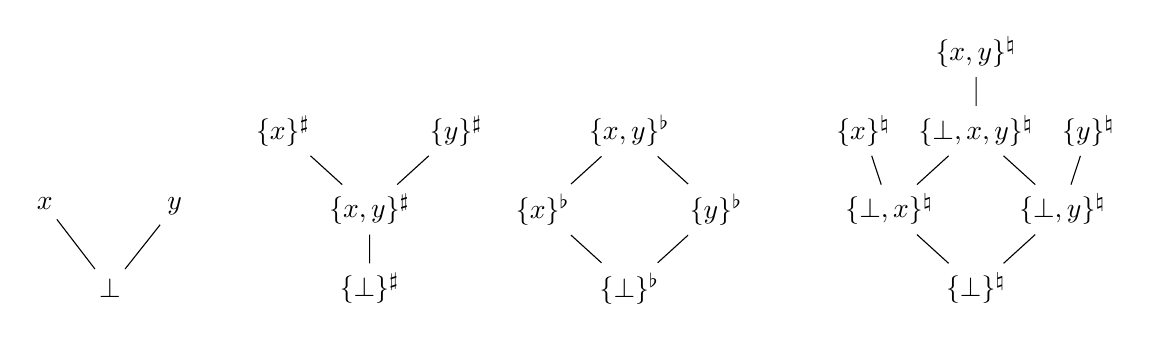
\begin{tikzpicture}[xscale=1.1]
  \node (U) at (0,0) {$\bot$};
  \node [anchor=base] (A) at (-0.75,1) {$x$};
  \node [anchor=base] (B) at (0.75,1) {$y$};
  \draw (A) -- (U) -- (B);
  
  \node (U1) at (3,0) {$\{\bot\}^\sharp$};
  \node (AB1) at (3,1) {$\{x,y\}^\sharp$};
  \node (A1) at (2,2) {$\{x\}^\sharp$};
  \node (B1) at (4,2) {$\{y\}^\sharp$};
  \draw (U1) -- (AB1);
  \draw (A1) -- (AB1) -- (B1);
  
  \node (U2) at (6,0) {$\{\bot\}^\flat$};
  \node (UA2) at (5,1) {$\{x\}^\flat$};
  \node (UAB2) at (6,2) {$\{x,y\}^\flat$};
  \node (UB2) at (7,1) {$\{y\}^\flat$};
  \draw (U2) -- (UA2) -- (UAB2);
  \draw (U2) -- (UB2) -- (UAB2);

  \node (U3) at (10,0) {$\{\bot\}^\natural$};
  \node (UA3) at (9,1) {$\{\bot,x\}^\natural$};
  \node (UB3) at (11,1) {$\{\bot,y\}^\natural$};
  \node (UAB3) at (10,2) {$\{\bot,x,y\}^\natural$};
  \node (A3) at (8.7,2) {$\{x\}^\natural$};
  \node (B3) at (11.3,2) {$\{y\}^\natural$};
  \node (AB3) at (10,3) {$\{x,y\}^\natural$};
  \draw (U3) -- (UA3) -- (A3);
  \draw (U3) -- (UB3) -- (B3);
  \draw (UA3) -- (UAB3);
  \draw (UB3) -- (UAB3);
  \draw (UAB3) -- (AB3);
\end{tikzpicture}
\par\end{centering}

\caption{Lifted two-element type, with upper, lower, and convex powerdomains}
\label{fig:lifted2}
\end{figure}


\begin{figure}
\begin{centering}
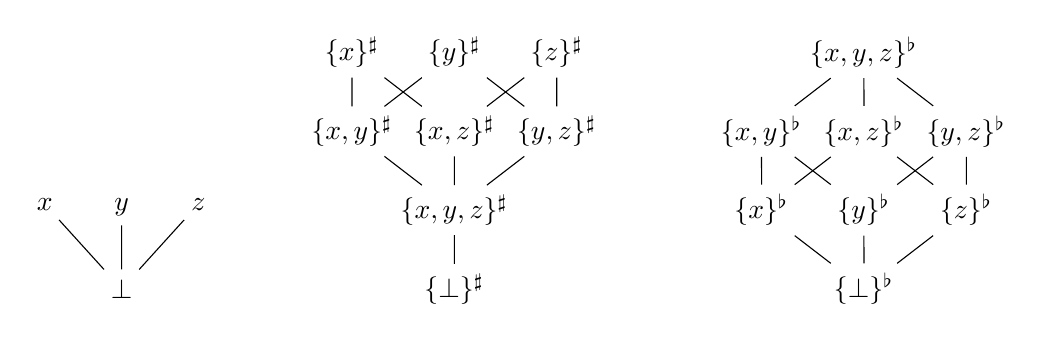
\begin{tikzpicture}[xscale=1.3]
  \node (U) at (0.75,0) {$\bot$};
  \node [anchor=base] (A) at (0,1) {$x$};
  \node [anchor=base] (B) at (0.75,1) {$y$};
  \node [anchor=base] (C) at (1.5,1) {$z$};
  \draw (U) -- (A);
  \draw (U) -- (B);
  \draw (U) -- (C);

  \node (U1) at (4,0) {$\{\bot\}^\sharp$};
  \node (ABC1) at (4,1) {$\{x,y,z\}^\sharp$};
  \node (AB1) at (3,2) {$\{x,y\}^\sharp$};
  \node (BC1) at (5,2) {$\{y,z\}^\sharp$};
  \node (CA1) at (4,2) {$\{x,z\}^\sharp$};
  \node (A1) at (3,3) {$\{x\}^\sharp$};
  \node (B1) at (4,3) {$\{y\}^\sharp$};
  \node (C1) at (5,3) {$\{z\}^\sharp$};
  \draw (U1) -- (ABC1);
  \draw (ABC1) -- (AB1) -- (A1) -- (CA1);
  \draw (ABC1) -- (BC1) -- (B1) -- (AB1);
  \draw (ABC1) -- (CA1) -- (C1) -- (BC1);

  \node (U2) at (8,0) {$\{\bot\}^\flat$};
  \node (UA2) at (7,1) {$\{x\}^\flat$};
  \node (UB2) at (8,1) {$\{y\}^\flat$};
  \node (UC2) at (9,1) {$\{z\}^\flat$};
  \node (UAB2) at (7,2) {$\{x,y\}^\flat$};
  \node (UBC2) at (9,2) {$\{y,z\}^\flat$};
  \node (UCA2) at (8,2) {$\{x,z\}^\flat$};
  \node (UABC2) at (8,3) {$\{x,y,z\}^\flat$};
  \draw (U2) -- (UA2) -- (UAB2);
  \draw (U2) -- (UB2) -- (UBC2);
  \draw (U2) -- (UC2) -- (UCA2);
  \draw (UA2) -- (UCA2) -- (UABC2);
  \draw (UB2) -- (UAB2) -- (UABC2);
  \draw (UC2) -- (UBC2) -- (UABC2);
\end{tikzpicture}
\par\end{centering}

\caption{Lifted three-element type, with upper and lower powerdomains}
\label{fig:lifted3}
\end{figure}


\begin{figure}
\begin{centering}
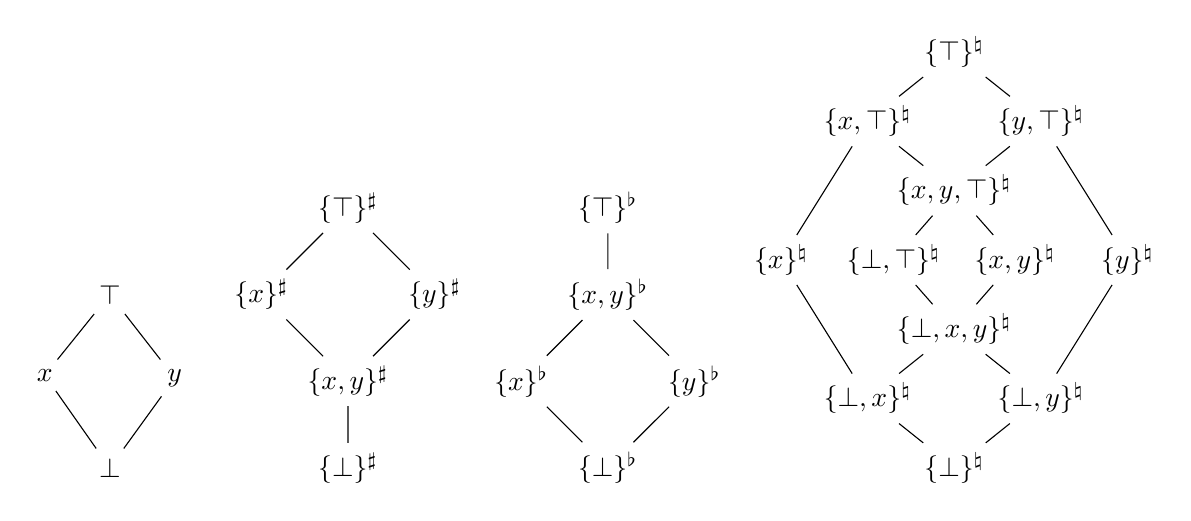
\begin{tikzpicture}[xscale=1.1, yscale=1.1]
  \node (U) at (1.25,0) {$\bot$};
  \node [anchor=base] (A) at (0.5,1) {$x$};
  \node [anchor=base] (B) at (2,1) {$y$};
  \node (T) at (1.25,2) {$\top$};
  \draw (U) -- (A) -- (T) -- (B) -- (U);
  
  \node (U1) at (4,0) {$\{\bot\}^\sharp$};
  \node (AB1) at (4,1) {$\{x,y\}^\sharp$};
  \node (A1) at (3,2) {$\{x\}^\sharp$};
  \node (B1) at (5,2) {$\{y\}^\sharp$};
  \node (T1) at (4,3) {$\{\top\}^\sharp$};
  \draw (U1) -- (AB1) -- (A1) -- (T1) -- (B1) -- (AB1);

  \node (U2) at (7,0) {$\{\bot\}^\flat$};
  \node (A2) at (6,1) {$\{x\}^\flat$};
  \node (B2) at (8,1) {$\{y\}^\flat$};
  \node (AB2) at (7,2) {$\{x,y\}^\flat$};
  \node (T2) at (7,3) {$\{\top\}^\flat$};
  \draw (T2) -- (AB2) -- (B2) -- (U2) -- (A2) -- (AB2);
  
  \node (U3) at (11,0) {$\{\bot\}^\natural$};
  \node (UA3) at (10,0.8) {$\{\bot,x\}^\natural$};
  \node (UB3) at (12,0.8) {$\{\bot,y\}^\natural$};
  \node (UAB3) at (11,1.6) {$\{\bot,x,y\}^\natural$};
  \node (A3) at (9,2.4) {$\{x\}^\natural$};
  \node (B3) at (13,2.4) {$\{y\}^\natural$};
  \node (UT3) at (10.3,2.4) {$\{\bot,\top\}^\natural$};
  \node (AB3) at (11.7,2.4) {$\{x,y\}^\natural$};
  \node (ABT3) at (11,3.2) {$\{x,y,\top\}^\natural$};
  \node (AT3) at (10,4.0) {$\{x,\top\}^\natural$};
  \node (BT3) at (12,4.0) {$\{y,\top\}^\natural$};
  \node (T3) at (11,4.8) {$\{\top\}^\natural$};
  \draw (U3) -- (UA3) -- (UAB3);
  \draw (U3) -- (UB3) -- (UAB3);
  \draw (UA3) -- (A3) -- (AT3);
  \draw (UB3) -- (B3) -- (BT3);
  \draw (UAB3) -- (UT3) -- (ABT3);
  \draw (UAB3) -- (AB3) -- (ABT3);
  \draw (ABT3) -- (AT3) -- (T3);
  \draw (ABT3) -- (BT3) -- (T3);
\end{tikzpicture}
\par\end{centering}
\caption{Four-element lattice, with upper, lower, and convex powerdomains}
\label{fig:lattice4}
\end{figure}


\section{Powerdomain library features}
\label{sec:HOLCF-powerdomain-library}

This section describes the user-visible aspects of the HOLCF powerdomain library. The implementation defines three new type constructors, one for each of the three powerdomain varieties. Each type has \isa{unit} and \isa{plus} constructors, and a monadic \isa{bind} operator. Each type also has \isa{map} and \isa{join} operators, defined in terms of \isa{unit} and \isa{bind} in the same manner as Haskell's \texttt{liftM} and \texttt{join}. The full list of types and constants is shown in Fig. \ref{fig:type-signatures}.

The functions \isa{convex_to_lower} and \isa{convex_to_upper} are the mappings guaranteed to exist by the universal property of the convex powerdomain; they preserve \isa{unit} and \isa{plus}. Note that instead of the full function space (\isa{=>}), all functions use the HOLCF continuous function space type (\isa{->}), indicating that they are continuous functions.

\begin{figure}
\indexdef{upper_unit}
\indexdef{upper_plus}
\indexdef{upper_bind}
\indexdef{upper_map}
\indexdef{upper_join}
\begin{isacode}
upper_unit :: 'a -> 'a upper_pd
upper_plus :: 'a upper_pd -> 'a upper_pd -> 'a upper_pd
upper_bind :: 'a upper_pd -> ('a -> 'b upper_pd) -> 'b upper_pd
upper_map :: ('a -> 'b) -> 'a upper_pd -> 'b upper_pd
upper_join :: 'a upper_pd upper_pd -> 'a upper_pd
\end{isacode}
\unmedskip
\indexdef{lower_unit}
\indexdef{lower_plus}
\indexdef{lower_bind}
\indexdef{lower_map}
\indexdef{lower_join}
\begin{isacode}
lower_unit :: 'a -> 'a lower_pd
lower_plus :: 'a lower_pd -> 'a lower_pd -> 'a lower_pd
lower_bind :: 'a lower_pd -> ('a -> 'b lower_pd) -> 'b lower_pd
lower_map :: ('a -> 'b) -> 'a lower_pd -> 'b lower_pd
lower_join :: 'a lower_pd lower_pd -> 'a lower_pd
\end{isacode}
\unmedskip
\indexdef{convex_unit}
\indexdef{convex_plus}
\indexdef{convex_bind}
\indexdef{convex_map}
\indexdef{convex_join}
\begin{isacode}
convex_unit :: 'a -> 'a convex_pd
convex_plus :: 'a convex_pd -> 'a convex_pd -> 'a convex_pd
convex_bind :: 'a convex_pd -> ('a -> 'b convex_pd) -> 'b convex_pd
convex_map :: ('a -> 'b) -> 'a convex_pd -> 'b convex_pd
convex_join :: 'a convex_pd convex_pd -> 'a convex_pd
\end{isacode}
\unmedskip
\indexdef{convex_to_upper}
\indexdef{convex_to_lower}
\begin{isacode}
convex_to_upper :: 'a convex_pd -> 'a upper_pd
convex_to_lower :: 'a convex_pd -> 'a lower_pd
\end{isacode}

\caption{Powerdomain constants defined in \HOLCF{11}}
\label{fig:type-signatures}
\end{figure}

For convenience, the library also provides set-style syntax for powerdomain operations: We can write \isa{\<lbrace>x\<rbrace>\<sharp>} for \isa{upper_unit\<cdot>x}, \isa{xs \<union>\<sharp> ys} for \isa{upper_plus\<cdot>xs\<cdot>ys}, \isa{\<Union>\<sharp>x\<in>xs. t} for \isa{upper_bind\<cdot>xs\<cdot>(\<Lambda> x. t)}, and so on for the other powerdomain types.

Along with the definitions of types and constants, the library provides a significant body of lemmas, many of which are declared to the simplifier. Each powerdomain type has an induction rule in terms of \isa{unit} and \isa{plus}, similar to Eq.~(\ref{eq:pd-induct}). Rules about injectivity, strictness, compactness, and ordering are provided for the constructors. Rewrite rules are provided for the \isa{bind}, \isa{map}, and \isa{join} functions applied to \isa{unit}, \isa{plus}, or \isa{\<bottom>}. All of the powerdomain laws are also included as lemmas.


\subsection{Type class constraints}
\label{sec:pd-class-constraint}

The main axiomatic type classes in HOLCF are \isa{cpo} (chain-complete partial orders) and \isa{pcpo} (pointed cpos). Unfortunately, the powerdomain constructions do not work over arbitrary cpos; they need some additional structure. To formalize powerdomains in HOLCF, it was necessary to add a new axiomatic class \isa{bifinite}, which is a subclass of \isa{pcpo}. All of the functions defined in the \HOLCF{11} powerdomain theories have a \isa{bifinite} class constraint. The definition and relevant properties of class \isa{bifinite} will be discussed in Section \ref{sec:pd-bifinite}.

As far as a user of the library is concerned, it does not matter how class \isa{bifinite} is defined; the important thing is that it should be preserved by all of type constructors that the user works with. \HOLCF{11} provides \isa{bifinite} class instances for all of its type constructors: continuous function space, cartesian product, strict product, strict sum, lifted cpos, and all three varieties of powerdomains. Flat domains built from countable HOL types are also instances of \isa{bifinite}. The \textsc{Domain} package also generates instances of the \isa{bifinite} class, when it is used in its definitional mode (see Chapter~\ref{ch:universal}).


\subsection{Automation}

To facilitate reasoning with powerdomains, the library provides various sets of rewrite rules that are designed to work well together.

\paragraph{ACI normalization.} Isabelle's simplifier is set up to handle permutative rewrite rules, which are equations like $x+y=y+x$ whose right and left-hand-sides are the same modulo renaming of variables \cite{isabelle-tutorial}. For any associative-commutative (AC) operator, there is a set of three permutative rewrite rules that can convert any expression built from the operator into a normal form (grouped to the right, with terms sorted according to some syntactic term-ordering) \cite{baader1998}. Two of the AC rewrites are simply the associativity and commutativity rules. The third is the left-commutativity rule. For normalizing an associative-commutative-idempotent (ACI) operator, we need a total of five rules: the three AC rewrites, plus the idempotency rule, and also (analogous to left-commutativity) left-idempotency.
\begin{eqnarray}
(xs\cup ys)\cup zs & = & xs\cup(ys\cup zs)\nonumber \\
ys\cup xs & = & xs\cup ys\nonumber \\
ys\cup(xs\cup zs) & = & xs\cup(ys\cup zs)\label{eq:plus-aci}\\
xs\cup xs & = & xs\nonumber \\
xs\cup(xs\cup ys) & = & xs\cup ys\nonumber
\end{eqnarray}

Permutative rewriting using the ACI rules results in a normal form where expressions are nested to the right, and the terms are sorted according to the syntactic term ordering, with no exact duplicates. In \HOLCF{11}, this normalization can be accomplished for the convex powerdomains by invoking the simplifier with \isa{simp add: convex_plus_aci}. Similarly, \isa{upper_plus_aci} and \isa{lower_plus_aci} may be used with upper and lower powerdomains, respectively.


\paragraph{Solving inequalities.} A common subgoal in a proof might be to show that one powerdomain expression is below another. For each variety of powerdomain, there is a set of rewrite rules that can automatically reduce an inequality on powerdomains down to inequalities on the underlying type.
\begin{eqnarray}
\{x\}^{\sharp}\sqsubseteq\{y\}^{\sharp} & \iff & x\sqsubseteq y\nonumber \\
xs\sqsubseteq(ys\cup^{\sharp}zs) & \iff & (xs\sqsubseteq ys)\wedge(xs\sqsubseteq zs)\label{eq:upper-less}\\
(xs\cup^{\sharp}ys)\sqsubseteq\{z\}^{\sharp} & \iff & (xs\sqsubseteq\{z\}^{\sharp})\vee(ys\sqsubseteq\{z\}^{\sharp})\nonumber
\end{eqnarray}
\begin{eqnarray}
\{x\}^{\flat}\sqsubseteq\{y\}^{\flat} & \iff & x\sqsubseteq y\nonumber \\
(xs\cup^{\flat}ys)\sqsubseteq zs & \iff & (xs\sqsubseteq zs)\wedge(ys\sqsubseteq zs)\label{eq:lower-less}\\
\{x\}^{\flat}\sqsubseteq(ys\cup^{\flat}zs) & \iff & (\{x\}^{\flat}\sqsubseteq ys)\vee(\{x\}^{\flat}\sqsubseteq zs)\nonumber
\end{eqnarray}
\begin{eqnarray}
\{x\}^{\natural}\sqsubseteq\{y\}^{\natural} & \iff & x\sqsubseteq y\nonumber \\
\{x\}^{\natural}\sqsubseteq(ys\cup^{\natural}zs) & \iff & (\{x\}^{\natural}\sqsubseteq ys)\wedge(\{x\}^{\natural}\sqsubseteq zs)\label{eq:convex-less}\\
(xs\cup^{\natural}ys)\sqsubseteq\{z\}^{\natural} & \iff & (xs\sqsubseteq\{z\}^{\natural})\wedge(ys\sqsubseteq\{z\}^{\natural})\nonumber
\end{eqnarray}

For the upper and lower powerdomains, each has a set of three rewrite rules that covers all cases of comparisons. For example, \isa{simp add: upper_pd_below_simps} will rewrite \isa{\<lbrace>x, y\<rbrace>\<sharp> \<sqsubseteq> \<lbrace>y, z\<rbrace>\<sharp>} into \isa{x \<sqsubseteq> z \<or> y \<sqsubseteq> z}, using the rules in Eq.~(\ref{eq:upper-less}). Similarly, simplification with \isa{lower_pd_below_simps} uses the rules in Eq.~(\ref{eq:lower-less}) to simplify inequalities on lower powerdomains.

For the convex powerdomain, the three rules in Eq.~(\ref{eq:convex-less}) are incomplete: They do not cover the case of $(xs\cup^{\natural}ys)\sqsubseteq(zs\cup^{\natural}ws)$. To handle this case, we will take advantage of the coercions from the convex powerdomain to the upper and lower powerdomains, along with the following ordering property:
%
\indexthm{convex_pd_below_iff}
\begin{isacode}
lemma convex_pd_below_iff:
  "(xs \<sqsubseteq> ys) <->
      (convex_to_upper\<cdot>xs \<sqsubseteq> convex_to_upper\<cdot>ys \<and>
        convex_to_lower\<cdot>xs \<sqsubseteq> convex_to_lower\<cdot>ys)"
\end{isacode}
%
The rule set \isa{convex_pd_below_simps} includes all rules from Eqs.~(\ref{eq:upper-less})--(\ref{eq:convex-less}), and a suitably instantiated \isa{convex_pd_below_iff} to cover the missing case.

\paragraph{Using inequalities to solve non-trivial equalities.} The ACI rewriting can take care of many equalities between powerdomain expressions, but the inequality rules can actually solve more. For example, using the assumptions $x \sqsubseteq y$ and $y \sqsubseteq z$, we will prove that $\{x, y, z\}^\natural = \{x, z\}^\natural$. By antisymmetry, we can rewrite this to the conjunction $(\{x,y,z\}^{\natural}\sqsubseteq\{x,z\}^{\natural})\wedge(\{x,z\}^{\natural}\sqsubseteq\{x,y,z\}^{\natural})$. Next, we can simplify with \isa{convex_pd_below_simps}, and this subgoal reduces to $(y\sqsubseteq x\vee y\sqsubseteq z)\wedge(x\sqsubseteq y\vee z\sqsubseteq y)$. Finally, this is easily discharged using the assumptions $x\sqsubseteq y$ and $y\sqsubseteq z$.


\section{Ideal completion}
\label{sec:pd-ideal-completion}

In Chapter~\ref{ch:holcf}, we defined various basic HOLCF types as subsets of other cpos, using the \textsc{Cpodef} package. Unfortunately, this is not possible for powerdomains. In such cases where \textsc{Cpodef} is not applicable, we want to minimize the proof effort for proving the completeness axioms and continuity of operations. One way to accomplish this is to define a cpo using \emph{ideal completion}.

The powerdomain construction used in HOLCF makes use of an alternative representation of cpos, where we just consider the set of compact (i.e., finite) values, rather than the whole cpo~\cite[\S2.2.6]{abramsky94domain}. (Refer to Sec.~\ref{sec:holcf-fix} for the HOLCF definition and properties of compactness.) For a certain class of cpos, called \emph{algebraic} cpos, every value can be expressed as the least upper bound of its compact approximants. This means that in an algebraic cpo $D$ the set of compact elements $K(D)$, together with the ordering on them, fully represents the entire cpo. We say that $K(D)$ forms a \emph{basis} for the cpo $D$, and that the entire cpo $D$ is a \emph{completion} of the basis.

To construct a new algebraic cpo by ideal completion, we can start by defining its basis. The ordering on the basis can be any partial order, not necessarily a complete partial order. The operations on the basis only need to be monotone, not necessarily continuous. (This is helpful because monotonicity is generally much easier to prove than continuity.)  The ideal completion process extends the basis with new infinite elements to give a cpo. Similarly, a process called \emph{continuous extension} lifts the monotone operations on the basis up to continuous functions on the new cpo.

The ideal completion process is formalized as a library in \HOLCF{11}; this section will describe the formalization, and show how to define new cpo types with it. Section~\ref{sec:pd-implementation} shows how it is used to define the powerdomain type constructors. The process is general enough to be useful for other cpos besides powerdomains; Chapter~\ref{ch:universal} will show how it is used to construct a universal domain.

\subsection{Preorders and ideals}

A \emph{preorder} is defined as a binary relation that is reflexive and transitive. Given a basis with a preorder relation $\left\langle B,\preceq\right\rangle$, we can construct an algebraic cpo by ideal completion. This is done by considering the set of ideals over the basis:

\begin{definition}
A set $S \subseteq B$ is an \emph{ideal} with respect to preorder relation
$(\preceq)$ if it has the following properties:
\begin{itemize*}
\item $S$ is nonempty: $\exists x.\: x\in S$
\item $S$ is downward-closed: $\forall x\: y.\: x\preceq y\longrightarrow y\in S\longrightarrow x\in S$
\item $S$ is directed (i.e., has an upper bound for any pair of elements):\\
 $\forall x\: y.\: x\in S\longrightarrow y\in S\longrightarrow(\exists z.\: z\in S\wedge x\preceq z\wedge y\preceq z)$
\end{itemize*}
A \emph{principal} \emph{ideal} is an ideal of the form $\{y \mid y\preceq x\}$ for some $x$, written $\downarrow\! x$.
\end{definition}
The set of all ideals over $\left\langle B,\preceq\right\rangle $ is denoted by $\mathrm{Idl}(B)$; when ordered by subset inclusion, $\mathrm{Idl}(B)$ forms an algebraic cpo. The compact elements of $\mathrm{Idl}(B)$ are exactly those represented by principal ideals. The algebraicity of $\mathrm{Idl}(B)$ is manifest in the following induction rule: For an admissible predicate $P$, if $P$ holds for all principal ideals, then it holds for all elements of $\mathrm{Idl}(B)$.
%
\begin{equation}
\inferrule
  {\mathrm{adm}(P) \\ \forall x \in B.\:P(\downarrow\! x)}
  {\forall y \in \mathrm{Idl}(B).\:P(y)}
\label{eq:ideal-induct}
\end{equation}
%
(If the notion of admissibility is defined using directed sets, then Eq.~\eqref{eq:ideal-induct} holds for any preordered basis $B$. But if admissibility is defined using countable chains---as it is in HOLCF---then we must require the basis $B$ to be a countable set.)

Note that we do not require $(\preceq)$ to be antisymmetric. For $x$ and $y$ that are equivalent (that is, both $x\preceq y$ and $y\preceq x$) the principal ideals $\downarrow\! x$ and $\downarrow\! y$ are equal. This means that the ideal completion construction automatically quotients by the equivalence induced by $(\preceq)$.

\subsection{Formalizing ideal completion}
\label{sec:pd-completion-formalize}

%Ideal completion is formalized using Isabelle's locale mechanism~\cite{KWP99locales, Ballarin10}. A \emph{locale} is essentially like a named proof context: It fixes parameters and collects assumptions about them. Lemmas can be proved \emph{in} a locale, where the assumptions of the locale become extra implicit hypotheses. Likewise, constants can be defined in a locale, and the locale parameters become extra implicit arguments. Locales can then be \emph{interpreted} by instantiating the parameters with values that satisfy the assumptions, generating customized versions of all the constants and lemmas from the locale.
Ideal completion is formalized using Isabelle's locale mechanism~\cite{KWP99locales, Ballarin10}. A \emph{locale} is like a named proof context: It fixes parameters and collects assumptions about them. Lemmas can be proved \emph{in} a locale, where the assumptions of the locale become extra implicit hypotheses. Likewise, constants can be defined in a locale, with the locale parameters as extra implicit arguments. Locales can be \emph{interpreted} by instantiating the parameters with values that satisfy the assumptions, generating specialized versions of all the constants and lemmas from the locale.

Locales are similar in some ways to axiomatic type classes. Both of these mechanisms are used to formalize algebraic structures, which involve some number of fixed operations and assumptions about them. However, each mechanism has its own strengths and limitations, and some situations require one or the other. The formalization of ideal completion relies on two features unique to locales: First, while a type class may only mention a single type variable, locales may be parameterized by any number of types. This feature is necessary because ideal completion relates two types: a basis and a completed cpo. Second, locales allow multiple interpretations at the same type---unlike type classes, which only allow one instantiation per type. This feature allows us to define multiple preorders and ideal completions with the same basis type.


\paragraph{Locale for preorders.} The \HOLCF{11} ideal completion library defines two locales, \isa{preorder} and \isa{ideal_completion}; we will discuss the \isa{preorder} locale first. The \isa{preorder} locale fixes a type \isa{'a} corresponding to the basis $B$, and a preorder relation \isa{\<preceq>} on that type. We also define a predicate \isa{ideal} within the locale.
%
\indexdef{preorder}
\begin{isacode}
locale preorder =
  fixes r :: "'a::type => 'a => bool" (infix "\<preceq>" 50)
  assumes r_refl: "x \<preceq> x"
  assumes r_trans: "[|x \<preceq> y; y \<preceq> z|] ==> x \<preceq> z"
\end{isacode}
\unmedskip
\indexdef{ideal}
\begin{isacode}
definition (in preorder) ideal :: "'a set => bool"
  where "ideal A \<longleftrightarrow>
    (\<exists>x. x \<in> A) \<and> (\<forall>x\<in>A. \<forall>y\<in>A. \<exists>z\<in>A. x \<preceq> z \<and> y \<preceq> z) \<and>
    (\<forall>x y. x \<preceq> y --> y \<in> A --> x \<in> A)"
\end{isacode}
%
Within the \isa{preorder} locale, we prove that principal ideals are indeed ideals. We also prove that the union of a chain of ideals is itself an ideal---which shows that the ideal completion is a cpo.
%
\indexthm{ideal_principal}
\begin{isacode}
lemma (in preorder) ideal_principal:
  shows "ideal {x. x \<preceq> z}"
\end{isacode}
\unmedskip
\indexthm{ideal_UN}
\begin{isacode}
lemma (in preorder) ideal_UN:
  fixes A :: "nat => 'a set"
  assumes ideal_A: "\<And>i. ideal (A i)"
  assumes chain_A: "\<And>i j. i \<le> j ==> A i \<subseteq> A j"
  shows "ideal (\<Union>i. A i)"
\end{isacode}
%
Next we shall consider the steps required to define a new cpo in Isabelle using ideal completion. The first step is to choose a type to use as a basis and define a preorder relation on it. For example, as a basis we might use lists of natural numbers, with a prefix ordering (\isa{@} is Isabelle's list-append operator). After defining the relation we proceed to interpret the \isa{preorder} locale.
%
\indexdefx{prefix}
\begin{isacode}
definition prefix :: "nat list => nat list => bool"
  where "prefix xs ys = (\<exists>zs. ys = xs @ zs)"
\end{isacode}
\unmedskip
\begin{isacode}
interpretation preord_prefix: preorder prefix
  by ...
\end{isacode}
%
The interpretation command requires a proof that \isa{prefix} satisfies the assumptions of the locale---in this case, reflexivity and transitivity. After we discharge the proof obligations, the locale package generates copies of all constants and lemmas from the \isa{preorder} locale, instantiated with \isa{prefix} in place of \isa{\<preceq>} and with the qualifier ``\isa{preord_prefix}'' prepended to all the names.

The next step is to define a new type as the set of ideals over the basis, using \textsc{Typedef}. (Recall that the \isa{open} option serves merely to prevent \textsc{Typedef} from defining an unneeded set constant called \isa{inflist}.) The non-emptiness obligation can be discharged using lemma \isa{preord_prefix.ideal_principal}.
%
\begin{isacode}
typedef (open) inflist = "{S::nat list set. preord_prefix.ideal S}"
\end{isacode}
%
After defining the type, we define the ordering \isa{(\<sqsubseteq>)} on type \isa{inflist} in terms of the subset ordering on type \isa{nat list set}.
%
\indexthmx{below_inflist_def}
\begin{isacode}
instantiation inflist :: below
begin
  definition below_inflist_def: "(x \<sqsubseteq> y) = (Rep_inflist x \<subseteq> Rep_inflist y)"
  instance ..
end
\end{isacode}
%
We still need to prove that \isa{inflist} is an instance of the \isa{po} and \isa{cpo} classes. For this purpose, the ideal completion library provides a pair of lemmas that are very similar to those used by the \textsc{Cpodef} package from Chapter~\ref{ch:holcf} (\S\ref{sec:holcf-cpodef}). They have assumptions about the \isa{type_definition} predicate, and their conclusions are \isa{OFCLASS} predicates.
%
\indexthm{typedef_ideal_po}
\begin{isacode}
lemma (in preorder) typedef_ideal_po:
  fixes Rep :: "'b::below => 'a set'' and Abs :: "'a set => 'b"
  assumes type: "type_definition Rep Abs {S. ideal S}"
  assumes below: "\<And>x y. x \<sqsubseteq> y \<longleftrightarrow> Rep x \<subseteq> Rep y"
  shows "OFCLASS('b, po_class)"
\end{isacode}
\unmedskip
\indexthm{typedef_ideal_cpo}
\begin{isacode}
lemma (in preorder) typedef_ideal_cpo:
  fixes Rep :: "'b::po => 'a set'' and Abs :: "'a set => 'b"
  assumes type: "type_definition Rep Abs {S. ideal S}"
  assumes below: "\<And>x y. x \<sqsubseteq> y \<longleftrightarrow> Rep x \<subseteq> Rep y"
  shows "OFCLASS('b, cpo_class)"
\end{isacode}
%
The proof of \isa{typedef_ideal_po} is straightforward. To prove \isa{typedef_ideal_cpo}, we show that \isa{Abs (\<Union>i. Rep (Y i))} gives the least upper bound for any chain \isa{Y}.

Using lemma \isa{type_definition_inflist} (provided by \textsc{Typedef}) and \isa{below_inflist_def} together with \isa{preord_prefix.typedef_ideal_po} and \isa{preord_prefix.typedef_ideal_cpo}, we can prove the \isa{po} and \isa{cpo} class instances for \isa{inflist}.

\paragraph{Locale for ideal completions.} Having defined a cpo with ideal completion, we can now define an embedding from the basis type into the completion type, using principal ideals.
%
\indexdefx{principal_inflist}
\begin{isacode}
definition principal_inflist :: "nat list => inflist"
  where "principal_inflist x = Abs_inflist {a. prefix a x}"
\end{isacode}
%
In order to prove generic theorems about this embedding, HOLCF defines another locale on top of the \isa{preorder} locale, called \isa{ideal_completion}. In addition to type \isa{'a} representing the basis $B$, the new locale fixes another type \isa{'b} corresponding to $\mathrm{Idl}(B)$. It fixes two new functions: \isa{rep} returns the representation of a value as a set of basis elements, generalizing the function \isa{Rep_inflist}; and \isa{principal} returns values that correspond to principal ideals, generalizing \isa{principal_inflist}.
%
\indexdef{ideal_completion}
\begin{isacode}
locale ideal_completion = preorder +
  fixes principal :: "'a::type \<Rightarrow> 'b::cpo"
  fixes rep :: "'b::cpo \<Rightarrow> 'a::type set"
  assumes ideal_rep: "\<And>x. ideal (rep x)"
  assumes rep_lub: "\<And>Y. chain Y \<Longrightarrow> rep (\<Squnion>i. Y i) = (\<Union>i. rep (Y i))"
  assumes rep_principal: "\<And>a. rep (principal a) = {b. b \<preceq> a}"
  assumes belowI: "\<And>x y. rep x \<subseteq> rep y \<Longrightarrow> x \<sqsubseteq> y"
  assumes countable: "\<exists>f::'a \<Rightarrow> nat. inj f"
\end{isacode}
%
The assumptions of the \isa{ideal_completion} locale are designed to be easily satisfied by types like \isa{inflist} that are defined by ideal completion over a countable basis type. To assist with \isa{ideal_completion} locale interpretation proofs, the library provides the following lemma:
%
\indexthm{typedef_ideal_completion}
\begin{isacode}
lemma (in preorder) typedef_ideal_completion:
  fixes Rep :: "'b::cpo => 'a set" and Abs :: "'a set => 'b"
  assumes type: "type_definition Rep Abs {S. ideal S}"
  assumes below: "\<And>x y. x \<sqsubseteq> y \<longleftrightarrow> Rep x \<subseteq> Rep y"
  assumes principal: "\<And>a. principal a = Abs {b. b \<preceq> a}"
  assumes countable: "\<exists>f::'a \<Rightarrow> nat. inj f"
  shows "ideal_completion r principal Rep"
\end{isacode}
%
Within the \isa{ideal_completion} locale, we start by proving a few simple lemmas about \isa{principal}: The ordering between principal values reflects the basis ordering, and every principal value is compact.
%
\indexthm{principal_below_iff}
\begin{isacode}
lemma (in ideal_completion) principal_below_iff [simp]:
  "principal a \<sqsubseteq> principal b <-> a \<preceq> b"
\end{isacode}
\unmedskip
\indexthm{compact_principal}
\begin{isacode}
lemma (in ideal_completion) compact_principal [simp]:
  "compact (principal a)"
\end{isacode}
%
Perhaps the most important theorem in the \isa{ideal_completion} locale, however, is the principal induction rule given in Eq.~\eqref{eq:ideal-induct}. In order to help prove it, we must start with a lemma related to the countability of the basis: Any value in the complete cpo can be expressed as the least upper bound of a chain of principal values.
%
\indexthm{obtain_principal_chain}
\begin{isacode}
lemma (in ideal_completion) obtain_principal_chain:
  "\<exists>Y. (\<forall>i. Y i \<preceq> Y (Suc i)) \<and> x = (\<Squnion>i. principal (Y i))"
\end{isacode}
%
The proof proceeds by explicitly constructing such a chain, following a technique from the proof of Proposition 2.2.14 in Abramsky and Jung \cite{abramsky94domain}. Let $(b_n)_{n\in\omega}$ be an enumeration of the basis $B$, and let $x$ be a value in the completion represented by the ideal $S$. Then we can construct a sequence of basis values $(s_i)_{i\in\omega}$ as follows. Let $s_0$ be the first $b_n$ such that $b_n \in S$. Then for every $i\in\omega$ we define $t_i$ as the first $b_n$ such that $b_n \in S$ and $b_n \not\preceq s_i$. Then we inductively define $s_{i+1}$ as the first $b_n$ in $S$ above both $s_i$ and $t_i$. It can be shown that the sequence $s_i$ yields the desired least upper bound.

Using lemma \isa{obtain_principal_chain}, the principal induction rule follows directly.
%
\vspace{-22pt} % FUDGE
\indexthm{principal_induct}
\begin{isacode}
lemma (in ideal_completion) principal_induct:
  "[|adm P; !!a. P (principal a)|] ==> P x"
\end{isacode}
%
As we will see later in Sec.~\ref{sec:pd-implementation}, induction over principal values is the primary way to transfer properties about the basis type up to the completed cpo. Lemma \isa{principal_induct} is used dozens of times in the proof scripts of the \HOLCF{11} powerdomain theories.

\subsection{Continuous extensions of functions}

A continuous function on an algebraic cpo is completely determined by its action on compact elements. This suggests a method for defining continuous functions over ideal completions: First, define a function from the basis $B$ to a cpo $C$ such that $f$ is monotone, i.e., $x\preceq y$ implies $f(x)\sqsubseteq f(y)$. Then there exists a unique function $\widehat{f}:\mathrm{Idl}(B)\rightarrow C$ that agrees with $f$ on principal ideals, i.e., for all $x$, $\widehat{f}(\downarrow\! x)=f(x)$. We say that $\widehat{f}$ is the \emph{continuous extension} of $f$.

The continuous extension is defined by mapping the function $f$ over the input ideal, and then taking the least upper bound of the resulting directed set: $\widehat{f}(S)=\bigsqcup_{x\in S}f(x)$. Generally, the result type $C$ would need to be a directed-complete partial order\footnote{Directed-completeness means that every directed set has a least upper bound. This is a stronger condition than chain-completeness, which is used in the HOLCF formalization of cpos.} to ensure that this least upper bound exists. However, if the basis $B$ is countable, then it is possible to find a chain in $S$ that yields the same least upper bound as $S$. This means that $C$ can be any chain-complete partial order.

\subsection{Formalizing continuous extensions}

Within the \isa{ideal_completion} locale we define a function \isa{extension}, which takes a monotone function $f$ as an argument, and returns the continuous extension $\widehat{f}$.
%
\indexdef{extension}
\begin{isacode}
definition (in ideal_completion) extension :: "('a \<Rightarrow> 'c::cpo) \<Rightarrow> ('b \<rightarrow> 'c)"
  where "extension f = (\<Lambda> x. lub (image f (rep x)))"
\end{isacode}
%
The definition of \isa{extension} uses two features that are only well-defined if certain conditions are met: First, the function \isa{lub} requires that its argument actually have a least upper bound. Second, the continuous function abstraction requires that the body be continuous in \isa{x}. Both of these properties rely on the monotonicity of \isa{f}.

To prove that \isa{image f (rep x)} has a least upper bound, we use the lemma \isa{obtain_principal_chain} to get a chain \isa{Y :: nat => 'a} of basis elements such that \isa{x =} \isa{(\<Squnion>i. principal (Y i))}. Then we show that \isa{(\<Squnion>i. f (Y i))} is the desired least upper bound. The continuity of the abstraction then follows from \isa{rep_lub} combined with properties of least upper bounds. Finally, we can establish the behavior of \isa{extension} on principal ideals, using the fact that \isa{f a} is a least upper bound of the set \isa{image f (rep (principal a))}.
%
\indexthm{extension_principal}
\begin{isacode}
lemma extension_principal:
  assumes f_mono: "\<And>a b. a \<preceq> b \<Longrightarrow> f a \<sqsubseteq> f b"
  shows "extension f\<cdot>(principal a) = f a"
\end{isacode}
%
To prove a property about a function defined as a continuous extension, the general approach is to use principal induction (lemma \isa{principal_induct}) to reduce the general subgoal to one about principal values; then lemma \isa{extension_principal} can be used to unfold the definition.

\section{Bifinite cpos}
\label{sec:pd-bifinite}

The construction used here for powerdomains only works with element types that are algebraic cpos, having bases of compact elements. As was mentioned earlier in Sec.~\ref{sec:pd-class-constraint}, the type classes \isa{cpo} and \isa{pcpo} are not sufficient to meet this requirement. Instead, the powerdomain libraries are based on the \isa{bifinite} class, which is a subclass of \isa{pcpo}.
%
\begin{definition}
A continuous function $f : D \to D$ is a \emph{deflation} if it is idempotent and below the identity function: $f \circ f = f \sqsubseteq \mathrm{Id}_D$. A \emph{finite deflation} is a deflation whose image is a finite set.
\end{definition}
%
\begin{definition}
Let $D$ be a cpo, and let $\mathcal{M}$ be the set of finite deflations over $D$. Then we say that $D$ is \emph{bifinite} if $\mathcal{M}$ is countable and directed with $\bigsqcup \mathcal{M} = \mathrm{Id}_D$.
\end{definition}

Given a deflation $f$ over a cpo $D$, the image of $f$ identifies a sub-cpo of $D$. Similarly, a finite deflation over $D$ identifies a finite poset that is a subset of $K(D)$. Intuitively then, a bifinite cpo is one that can be expressed as the limit (in an appropriate sense) of a countable collection of finite posets.

A few notes on terminology: The definitions of ``deflation'' and ``finite deflation'' used here were taken from Gunter \cite[\S3.1]{gunter85thesis}. Deflations are also commonly known as ``projections'' or sometimes ``kernel operators'' \cite{abramsky94domain}. Abramsky and Jung also use the term ``idempotent deflation'' to refer to finite deflations \cite{abramsky94domain}. We include a countability requirement in the definition of bifiniteness, following Gunter and Scott \cite{gunter90semantic}. Some authors \cite{abramsky94domain} relax this requirement, allowing bifinite domains of arbitrary cardinality, and using the qualifiers ``countably based'' or ``$\omega$-bifinite'' as required. Bifinite domains were originally defined by Plotkin as limits of expanding sequences of finite posets, who used the name ``SFP domains''~\cite{plotkin76powerdomain}.

Many categories of cpos can be found in the domain theory literature \cite{amadio+curien, gunter90semantic, abramsky94domain}. Of all the possibilities, the bifinites were chosen because they meet the following criteria:
%
\begin{itemize}
\item All bifinite cpos are algebraic: Every bifinite type has a basis of compact elements, given by the union of the ranges of the finite deflations.
\item In bifinite cpos, every directed set contains a countable chain with the same limit. This means that for bifinite cpos, the notions of directed-continuity and chain-continuity coincide. This is important for fitting the ideal completion construction (which uses directed sets) into HOLCF (which defines everything with chains).
\item The class of bifinite cpos is closed under all type constructors used in HOLCF, including all three powerdomains.
\item A universal bifinite domain exists, which can be used to represent general recursive data\-types (see Chapter~\ref{ch:universal}).
\end{itemize}
%
The requirement for algebraicity rules out the chain-complete cpos (classes \isa{cpo} and \isa{pcpo}). The category of countably-based algebraic cpos meets the first two criteria, but it fails the third: The continuous function space between two arbitrary algebraic cpos is not necessarily algebraic. The category of bounded-complete domains (also known as ``Scott domains'') meets nearly all of the criteria, including having a universal domain---except that bounded-completeness fails to be preserved by the convex powerdomain \cite{gunter90semantic}.

\subsection{Type class for bifinite cpos}

Next we will see how the class \isa{bifinite} is defined in \HOLCF{11}. We start by defining \isa{deflation} and \isa{finite_deflation}. Defining them as locales makes it more convenient to prove numerous simple lemmas about deflations and finite deflations.
%
\indexdef{deflation}
\indexthm{deflation.idem}
\indexthm{deflation.below}
\begin{isacode}
locale deflation =
  fixes d :: "'a \<rightarrow> 'a"
  assumes idem: "\<And>x. d\<cdot>(d\<cdot>x) = d\<cdot>x"
  assumes below: "\<And>x. d\<cdot>x \<sqsubseteq> x"
\end{isacode}
\unmedskip
\indexdef{finite_deflation}
\indexthm{finite_fixes}
\begin{isacode}
locale finite_deflation = deflation +
  assumes finite_fixes: "finite {x. d\<cdot>x = x}"
\end{isacode}
%
Note that \isa{finite_deflation} is defined using the set of fixed points of \isa{d}, rather than the image of \isa{d}; it is provable within the \isa{deflation} locale that these sets are equal. This formulation makes it slightly easier to prove that particular functions are finite deflations.

For class \isa{bifinite}, instead of asserting directly that the collection of all finite deflations is countable and directed, we assume the existence of a countable chain of them whose least upper bound is the identity. Defining bifiniteness this way in terms of \isa{approx_chain} is convenient because we will be able to reuse it later: For the universal domain presented in Chapter~\ref{ch:universal}, embedding functions will be constructed within the \isa{approx_chain} locale.
%
\indexdef{approx_chain}
\indexthm{chain_approx}
\indexthm{lub_approx}
\indexthm{finite_deflation_approx}
\begin{isacode}
locale approx_chain =
  fixes approx :: "nat \<Rightarrow> 'a \<rightarrow> 'a"
  assumes chain_approx: "chain (\<lambda>i. approx i)"
  assumes lub_approx: "(\<Squnion>i. approx i) = ID"
  assumes finite_deflation_approx: "\<And>i. finite_deflation (approx i)"
\end{isacode}
\unmedskip
\indexdef{class bifinite}
\indexthm{bifinite}
\begin{isacode}
class bifinite = pcpo +
  assumes bifinite: "\<exists>a. approx_chain a"
\end{isacode}
%
To prove instances of the \isa{bifinite} class, we rely on a collection of map functions for each type constructor. Map functions were discussed previously in Chapter~\ref{ch:domain}, in the context of the \textsc{Domain} package (Fig.~\ref{fig:domain-map-combinators} gives a complete list). We repeat the definition of the map function for the product type:
%
\indexdef{prod_map}
\begin{isacode}
definition prod_map :: "('a \<rightarrow> 'b) \<rightarrow> ('c \<rightarrow> 'd) \<rightarrow> 'a \<times> 'c \<rightarrow> 'b \<times> 'd"
  where "prod_map = (\<Lambda> f g (x, y). (f\<cdot>x, g\<cdot>y))"
\end{isacode}
%
The \isa{prod_map} function applied to identity functions yields the identity function on pairs. We can also show that \isa{prod_map} applied to finite deflations yields a finite deflation.
%
\indexthm{prod_map_ID}
\begin{isacode}
lemma prod_map_ID:
  shows "prod_map\<cdot>ID\<cdot>ID = ID"
\end{isacode}
\unmedskip
\indexthm{finite_deflation_prod_map}
\begin{isacode}
lemma finite_deflation_prod_map:
  assumes "finite_deflation d1" and "finite_deflation d2"
  shows "finite_deflation (prod_map\<cdot>d1\<cdot>d2)"
\end{isacode}
%
A consequence of these properties is that \isa{prod_map} takes approx-chains to approx-chains, which is sufficient to show that the product type constructor preserves bifiniteness. Similarly, other map functions are used to prove \isa{bifinite} class instances for other basic HOLCF types (strict sums and products, continuous function space, and lifted cpos). Flat lifted HOL types like \isa{nat lift} are bifinite only if they are countable.

\subsection{Bifinite types as ideal completions}

Every bifinite cpo $D$ has a countable basis $K(D)$ of compact elements, of which $D$ is isomorphic to the ideal completion: $D \cong \mathrm{Idl}(K(D))$. Accordingly, we can create a locale interpretation that lets us treat types in class \isa{bifinite} as ideal completions. We define a partial order \isa{'a compact_basis} isomorphic to the set of compact elements of type \isa{'a}. The type \isa{'a compact_basis} will serve as the basis $K(D)$ while the original type \isa{'a} serves as $\mathrm{Idl}(K(D))$. The \isa{Rep_compact_basis} function from the type definition fills the role of the function \isa{principal} from the \isa{ideal_completion} locale. We define a function \isa{approximants} to act as the \isa{rep} function.
%
\indexdef{typedef 'a compact_basis}
\begin{isacode}
typedef (open) 'a compact_basis = "{x::('a::bifinite). compact x}"
\end{isacode}
\unmedskip
\indexdef{approximants}
\begin{isacode}
definition approximants :: "'a::bifinite => 'a compact_basis set"
  where "approximants x = {a. Rep_compact_basis a \<sqsubseteq> x}"
\end{isacode}
\unmedskip
\begin{isacode}
interpretation compact_basis:
  ideal_completion below Rep_compact_basis approximants
\end{isacode}
%
The proof of the locale interpretation is mostly straightforward; the trickiest part is proving that \isa{approximants x} is a directed set. For the proof, we apply rule \isa{bifinite} to obtain a chain of \isa{approx} functions, and use a lemma proved within the \isa{approx_chain} locale: A value is compact if and only if it is in the range of one of the \isa{approx} functions. To show directedness of \isa{approximants x}, let \isa{a} and \isa{b} be compact values below \isa{x}. Then there exist \isa{i} and \isa{j} such that \isa{approx i`a = a} and  \isa{approx j`b = b}. Finally, with a bit more work we can show that \isa{approx (max i j)`x} is a compact value below \isa{x} and above \isa{a} and \isa{b}.

Countability of the type \isa{'a compact_basis} also derives from the compactness rule. The set of compact values of type \isa{'a} is the union of the images of \isa{approx} functions. As a countable union of finite sets, it is also countable.\footnote{The proof of this fact requires the axiom of choice. Reliance on AC could be avoided by making an explicit enumeration of the basis part of the \isa{bifinite} class, but it is not clear that it would be worth the trouble to do so.}

\section{Construction of powerdomains}
\label{sec:pd-implementation}

All three of the powerdomains in the library are defined by ideal completion, following the construction given by Gunter and Scott~\cite[\S5.2]{gunter90semantic}. Each powerdomain uses the same basis type. If the algebraic cpo $D$ is the element type, then the powerdomain basis consists of nonempty, finite sets of compact elements of $D$. Formally, we would write this as $\mathcal{P}_f^*(K(D))$, where $K(D)$ is the compact basis of $D$, and $\mathcal{P}_f^*(S)$ denotes the set of finite, non-empty subsets of set $S$.

The lower, upper, and convex powerdomains all use the same basis, but each uses a different preorder relation:
\begin{eqnarray}
a\preceq^{\flat}b & \iff & \forall x\in a.\ \exists y\in b.\ x\sqsubseteq y\nonumber \\
a\preceq^{\sharp}b & \iff & \forall y\in b.\ \exists x\in a.\ x\sqsubseteq y\label{eq:preorders}\\
a\preceq^{\natural}b & \iff & a\preceq^{\flat}b\wedge a\preceq^{\sharp}b\nonumber
\end{eqnarray}
%
Note that these definitions are consistent with the characteristic ordering properties of powerdomains: We have $a \cup b \preceq^{\sharp} a$ in accordance with Eq.~\eqref{eq:upper-plus}, and $a \preceq^{\flat} a \cup b$ in accordance with Eq.~\eqref{eq:lower-plus}.

The various powerdomain operations, including unit, plus, and bind, are all defined as continuous extensions: In particular, the unit operation is the extension of the singleton function $\{-\} : K(D) \to \mathcal{P}_f^*(K(D))$, and plus is the extension of the union operation on $\mathcal{P}_f^*(K(D))$. Properties about all the functions can be derived using principal induction, as in Eq.~\eqref{eq:ideal-induct}.

The remainder of this section shows how these constructions are formalized in \HOLCF{11}. We start with the powerdomain basis type (\S\ref{sec:pd-basis}), and then define powerdomain types by ideal completion using the various preorders (\S\ref{sec:pd-typedef}). Next we define the constructors unit and plus by continuous extension (\S\ref{sec:pd-constructors}) and prove properties about them by induction (\S\ref{sec:pd-proofs}). Finally we define bind, map, and join functions and prove bifiniteness of the powerdomain types (\S\ref{sec:pd-monad}).

\subsection{Powerdomain basis type}
\label{sec:pd-basis}

To use as a basis for the various powerdomains, the library defines a type \isa{'a pd_basis}, which consists of nonempty, finite sets of elements of type \isa{'a compact_basis}. The constructor functions \isa{PDUnit} and \isa{PDPlus} build singleton sets and unions, respectively.
%
\indexdef{typedef 'a pd_basis}
\begin{isacode}
typedef 'a pd_basis = "{S::'a compact_basis set. finite S \<and> S \<noteq> {}}"
\end{isacode}
\unmedskip
\indexdef{PDUnit}
\begin{isacode}
definition PDUnit :: "'a compact_basis => 'a pd_basis"
  where "PDUnit x = Abs_pd_basis {x}"
\end{isacode}
\unmedskip
\indexdef{PDPlus}
\begin{isacode}
definition PDPlus :: "'a pd_basis => 'a pd_basis => 'a pd_basis"
  where "PDPlus t u = Abs_pd_basis (Rep_pd_basis t \<union> Rep_pd_basis u)"
\end{isacode}
%
Using the induction principle for finite sets from Isabelle's standard library, we derive an induction rule for the \isa{'a pd_basis} type, expressed in terms of the constructors.
%
\indexthm{pd_basis_induct}
\begin{isacode}
lemma pd_basis_induct:
  assumes PDUnit: "\<And>a. P (PDUnit a)"
  assumes PDPlus: "\<And>t u. \<lbrakk>P t; P u\<rbrakk> \<Longrightarrow> P (PDPlus t u)"
  shows "P x"
\end{isacode}
%
For defining operations like map, bind, and join, we also need the following fold operation on type \isa{'a pd_basis}. Its definition uses a finite-set fold operator \isa{fold1} provided by the standard Isabelle libraries \cite{Nipkow05}. Given an argument built from combinations of \isa{PDUnit} and \isa{PDPlus}, the function \isa{fold_pd g f} replaces \isa{PDUnit} with \isa{g} and \isa{PDPlus} with \isa{f}---but it is only well-defined if \isa{f} is associative, commutative, and idempotent.
%
\indexdef{fold_pd}
\begin{isacode}
definition fold_pd ::
    "('a compact_basis \<Rightarrow> 'b) \<Rightarrow> ('b \<Rightarrow> 'b \<Rightarrow> 'b) \<Rightarrow> 'a pd_basis \<Rightarrow> 'b"
  where "fold_pd g f t = fold1 f (image g (Rep_pd_basis t))"
\end{isacode}
%
Finally, using the countability of type \isa{'a compact_basis}, we prove that \isa{'a pd_basis} is a countable type as well. The proof uses an isomorphism between the natural numbers $\mathbb{N}$ and finite sets of naturals $\mathcal{P}_f(\mathbb{N})$, which is provided in the standard Isabelle libraries.

\subsection{Defining powerdomain types with ideal completion}
\label{sec:pd-typedef}

We will consider the definition of the upper powerdomain in some detail; the definitions of the other two powerdomain types are very similar. Having already defined the basis type, the next step is to define the preorder relation.
%
\begin{isacode}
definition upper_le :: "'a pd_basis \<Rightarrow> 'a pd_basis \<Rightarrow> bool" (infix "\<le>\<sharp>" 50)
  where "u \<le>\<sharp> v = (\<forall>y \<in> Rep_pd_basis v. \<exists>x \<in> Rep_pd_basis u. x \<sqsubseteq> y)"
\end{isacode}
\unmedskip
\begin{isacode}
interpretation upper_le: preorder upper_le
\end{isacode}
%
We follow the same process shown above in Sec.~\ref{sec:pd-completion-formalize}
for \isa{inflist} to define the type, instantiate \isa{po} and \isa{cpo} classes, and finally interpret the \isa{ideal_completion} locale. The complete code for this process is shown in Fig.~\ref{fig:pd-upper}.

\begin{figure}
\begin{isacode}
typedef (open) 'a upper_pd = "{S::'a pd_basis set. upper_le.ideal S}"
  by (auto intro: upper_le.ideal_principal)
\end{isacode}
\unmedskip
\indexdef{upper_principal}
\begin{isacode}
instantiation upper_pd :: (bifinite) below
begin
  definition "(x \<sqsubseteq> y) = (Rep_upper_pd x \<subseteq> Rep_upper_pd y)"
  instance ..
end
\end{isacode}
\unmedskip
\begin{isacode}
instance upper_pd :: (bifinite) po
  using type_definition_upper_pd below_upper_pd_def
  by (rule upper_le.typedef_ideal_po)
\end{isacode}
\unmedskip
\begin{isacode}
instance upper_pd :: (bifinite) cpo
  using type_definition_upper_pd below_upper_pd_def
  by (rule upper_le.typedef_ideal_cpo)
\end{isacode}
\unmedskip
\begin{isacode}
definition upper_principal :: "'a pd_basis \<Rightarrow> 'a upper_pd"
  where "upper_principal t = Abs_upper_pd {u. u \<le>\<sharp> t}"
\end{isacode}
\unmedskip
\begin{isacode}
interpretation upper_pd: ideal_completion upper_le upper_principal Rep_upper_pd
  using type_definition_upper_pd below_upper_pd_def
  using upper_principal_def pd_basis_countable
  by (rule upper_le.typedef_ideal_completion)
\end{isacode}
\caption{Defining the upper powerdomain type by ideal completion}
\label{fig:pd-upper}
\end{figure}

After proving the class instances and locale interpretations, we get to our first interesting proof: We can prove that type \isa{'a upper_pd} is pointed.
%
\begin{isacode}
lemma upper_pd_minimal:
  "upper_principal (PDUnit (Abs_compact_basis \<bottom>)) \<sqsubseteq> ys"
\end{isacode}
%
The proof is by induction on \isa{ys} using rule \isa{upper_pd.principal_induct}, which is one of the theorems generated by the locale interpretation.

\subsection{Defining constructor functions by continuous extension}
\label{sec:pd-constructors}

The \isa{extension} operators are used to define the powerdomain constructors \isa{upper_unit} and \isa{upper_plus} in terms of the singleton and union operations on the \isa{pd_basis} type. The function \isa{upper_unit} has an argument type of \isa{'a}, which uses \isa{'a compact_basis} as its basis type. Accordingly, we must use the \isa{extension} combinator from the \isa{compact_basis} locale interpretation to define it.
%
\indexdef{upper_unit}
\begin{isacode}
definition upper_unit :: "'a \<rightarrow> 'a upper_pd"
  where "upper_unit =
    compact_basis.extension (\<lambda>a. upper_principal (PDUnit a))"
\end{isacode}
%
The next step is to use the theorem \isa{compact_basis.extension_principal} to establish how \isa{upper_unit} acts on principal inputs. This requires a proof that the argument to \isa{compact_basis.extension} is monotone. Monotonicity is easy to show, because \isa{a \<sqsubseteq> b} implies \isa{PDUnit a \<le>\<sharp> PDUnit b}, which in turn implies \isa{upper_principal (PDUnit a) \<sqsubseteq>} \isa{upper_principal (PDUnit b)}.
%
\indexthm{upper_unit_Rep_compact_basis}
\begin{isacode}
lemma upper_unit_Rep_compact_basis [simp]:
  "upper_unit\<cdot>(Rep_compact_basis a) = upper_principal (PDUnit a)"
\end{isacode}
%
Unlike \isa{upper_unit}, the operator \isa{upper_plus} takes arguments of type \isa{'a upper_pd}, so we must define it using the \isa{extension} combinator from the \isa{upper_pd} locale. Because it takes two arguments, we nest two applications of \isa{upper_pd.extension}.
%
\indexdef{upper_plus}
\begin{isacode}
definition upper_plus :: "'a upper_pd \<rightarrow> 'a upper_pd \<rightarrow> 'a upper_pd"
  where "upper_plus = upper_pd.extension (\<lambda>t.
    upper_pd.extension (\<lambda>u. upper_principal (PDPlus t u)))"
\end{isacode}
%
Again, we prove how the constructor acts on principal inputs by showing monotonicity; here we must prove that the definition is monotone in both arguments. The proof obligation reduces to showing that \isa{PDPlus} is monotone with respect to \isa{\<le>\<sharp>}, which is easily proved by unfolding the definitions.
%
\indexthm{upper_plus_principal}
\begin{isacode}
lemma upper_plus_principal [simp]:
  "upper_plus\<cdot>(upper_principal t)\<cdot>(upper_principal u) =
    upper_principal (PDPlus t u)"
\end{isacode}
%
As mentioned earlier in Sec.~\ref{sec:HOLCF-powerdomain-library}, we introduce syntax for the constructors: \isa{\<lbrace>x\<rbrace>\<sharp>} for \isa{upper_unit\<cdot>x} and \isa{xs \<union>\<sharp> ys} for \isa{upper_plus\<cdot>xs\<cdot>ys}.

\subsection{Proving properties about the constructors}
\label{sec:pd-proofs}

After defining the constructor functions \isa{upper_unit} and \isa{upper_plus}, we must prove some properties about them. For example, we need to show that \isa{upper_plus} satisfies the powerdomain laws of associativity, commutativity, and idempotence. We must also prove the characteristic ordering property of upper powerdomains from Eq.~\eqref{eq:upper-plus}. These lemmas are all listed in Fig.~\ref{fig:pd-lemmas-easy}, and they all have similar proofs. Because each proposition is admissible in each variable (see Fig.~\ref{fig:holcf-adm-simps} from Sec.~\ref{sec:holcf-fix}), we can perform principal induction with rule \isa{upper_pd.principal_induct} to reduce them to propositions about elements of the basis: After applying induction and simplifying, \isa{(\<union>\<sharp>)} is replaced by \isa{PDPlus}, and \isa{(\<sqsubseteq>)} by \isa{(\<le>\<sharp>)}. The corresponding properties on the basis are then easy to show by unfolding the relevant definitions.

\begin{figure}
\indexthm{upper_plus_assoc}
\begin{isacode}
lemma upper_plus_assoc: "(xs \<union>\<sharp> ys) \<union>\<sharp> zs = xs \<union>\<sharp> (ys \<union>\<sharp> zs)"
\end{isacode}
\unmedskip
\indexthm{upper_plus_commute}
\begin{isacode}
lemma upper_plus_commute: "xs \<union>\<sharp> ys = ys \<union>\<sharp> xs"
\end{isacode}
\unmedskip
\indexthm{upper_plus_absorb}
\begin{isacode}
lemma upper_plus_absorb: "xs \<union>\<sharp> xs = xs"
\end{isacode}
\unmedskip
\indexthm{upper_plus_below1}
\begin{isacode}
lemma upper_plus_below1: "xs \<union>\<sharp> ys \<sqsubseteq> xs"
\end{isacode}
\unmedskip
\indexthm{upper_pd_induct}
\begin{isacode}
lemma upper_pd_induct:
  assumes P: "adm P"
  assumes unit: "\<And>x. P {x}\<sharp>"
  assumes plus: "\<And>xs ys. \<lbrakk>P xs; P ys\<rbrakk> \<Longrightarrow> P (xs \<union>\<sharp> ys)"
  shows "P (xs::'a upper_pd)"
\end{isacode}
\caption{Powerdomain lemmas with simple proofs by principal induction}
\label{fig:pd-lemmas-easy}
\end{figure}

The proof of the induction rule \isa{upper_pd_induct} starts the same way, with principal induction. This reduces the goal \isa{P xs} to one of the form \isa{P (upper_principal t)} for arbitrary \isa{t}. The proof then proceeds by induction on \isa{t} using rule \isa{pd_basis_induct}.

Other properties, such as the rewrite rules for comparisons from Eqs.~\eqref{eq:upper-less}--\eqref{eq:convex-less}, are a bit trickier to prove. Because they contain implications, which do not preserve admissibility, the principal induction rules are not so straightforward to apply. For example, consider the lemma \isa{upper_unit_below_iff} from Fig.~\ref{fig:pd-lemmas-tricky}. One direction of the equivalence can be solved by monotonicity, but this still leaves the implication \isa{\<lbrace>x\<rbrace>\<sharp> \<sqsubseteq> \<lbrace>y\<rbrace>\<sharp> --> x \<sqsubseteq> y}, which is equivalent to \isa{\<lbrace>x\<rbrace>\<sharp> \<notsqsubseteq> \<lbrace>y\<rbrace>\<sharp> \<or> x \<sqsubseteq> y}. Due to the negated comparison, this predicate is admissible in \isa{x} but not in \isa{y}. To complete the proof we will need to perform induction on both variables, but at first it seems we are stuck.

\begin{figure}
\indexthm{upper_unit_below_iff}
\begin{isacode}
lemma upper_unit_below_iff [simp]:
  "{x}\<sharp> \<sqsubseteq> {y}\<sharp> \<longleftrightarrow> x \<sqsubseteq> y"
\end{isacode}
\unmedskip
\indexthm{upper_plus_below_unit_iff}
\begin{isacode}
lemma upper_plus_below_unit_iff [simp]:
  "xs \<union>\<sharp> ys \<sqsubseteq> {z}\<sharp> \<longleftrightarrow> xs \<sqsubseteq> {z}\<sharp> \<or> ys \<sqsubseteq> {z}\<sharp>"
\end{isacode}
\caption{Powerdomain lemmas with tricky proofs by principal induction}
\label{fig:pd-lemmas-tricky}
\end{figure}

The solution involves using the admissibility rules for compactness from Chapter~\ref{ch:holcf}, specifically lemma \isa{adm_compact_not_below} from Fig.~\ref{fig:holcf-compact-simps}. Because the proposition is admissible in \isa{x}, we do principal induction on \isa{x} first; this replaces each occurrence of \isa{x} in the goal with \isa{Rep_compact_basis a}, for an arbitrary \isa{a}. The new subgoal now looks like this:
%
\begin{isacode}
\<lbrace>Rep_compact_basis a\<rbrace>\<sharp> \<sqsubseteq> \<lbrace>y\<rbrace>\<sharp> --> Rep_compact_basis a \<sqsubseteq> y
\end{isacode}
%
The original proposition with \isa{x} was not admissible in \isa{y}, but the new proposition is, because \isa{\<lbrace>Rep_compact_basis a\<rbrace>\<sharp>} is compact (it equals \isa{upper_principal (PDUnit a)}). This means we can proceed with a second principal induction on \isa{y}; the remainder of the proof is easy.

We use a similar proof strategy for lemma \isa{upper_plus_below_unit_iff}. The proposition of that lemma is admissible in \isa{xs} and \isa{ys}, but not in \isa{z}. But after doing principal induction on both \isa{xs} and \isa{ys}, replacing them respectively with \isa{upper_principal t} and \isa{upper_principal u}, we can use lemma \isa{adm_compact_not_below} to show that the remaining subgoal is admissible in \isa{z}. Most of the lemmas corresponding to Eqs.~(\ref{eq:upper-less})--(\ref{eq:convex-less}) use a similar proof, as does the \isa{convex_pd_below_iff} lemma, which also has an if-and-only-if form.

\subsection{Defining functor and monad operations}
\label{sec:pd-monad}

The \isa{upper_bind}, \isa{upper_map}, and \isa{upper_join} operations remain to be defined. Instead of defining each of these separately using continuous extension, it will be easiest to simply define the map and join operations in terms of \isa{upper_bind}. For the bind operation, we start by defining a function \isa{upper_bind_basis} that specifies how \isa{upper_bind} should behave on compact inputs.
%
\indexdef{upper_bind_basis}
\begin{isacode}
definition upper_bind_basis ::
    "'a pd_basis \<Rightarrow> ('a \<rightarrow> 'b upper_pd) \<rightarrow> 'b upper_pd"
  where "upper_bind_basis =
    fold_pd (\<lambda>a. \<Lambda> f. f\<cdot>(Rep_compact_basis a)) (\<lambda>x y. \<Lambda> f. x\<cdot>f \<union>\<sharp> y\<cdot>f)"
\end{isacode}
%
We must show that the second argument to \isa{fold_pd} is associative, commutative, and idempotent before we can derive the characteristic equations. These conditions follow directly from the lemmas shown in Fig.~\ref{fig:pd-lemmas-easy}.
%
\indexthm{upper_bind_basis_simps}
\begin{isacode}
lemma upper_bind_basis_simps:
  "upper_bind_basis (PDUnit a) = (\<Lambda> f. f\<cdot>(Rep_compact_basis a))"
  "upper_bind_basis (PDPlus t u) =
    (\<Lambda> f. upper_bind_basis t\<cdot>f \<union>\<sharp> upper_bind_basis u\<cdot>f)"
\end{isacode}
%
Next, \isa{upper_bind} is defined as the continuous extension of \isa{upper_bind_basis}. The proof that \isa{upper_bind_basis} is monotonic, i.e.\ that \isa{t \<le>\<sharp> u} implies \isa{upper_bind_basis t} \isa{\<sqsubseteq> upper_bind_basis u}, proceeds by induction on \isa{u}, and relies on \isa{upper_plus_below1} from Fig.~\ref{fig:pd-lemmas-easy}.
%The proof of monotonicity for \isa{upper_bind_basis}, showing that \isa{t \<le>\<sharp> u} implies \isa{upper_bind_basis t \<sqsubseteq> upper_bind_basis u} proceeds by induction on \isa{u}, and relies on \isa{upper_plus_below1} from Fig.~\ref{fig:pd-lemmas-easy}.
%
\indexdef{upper_bind}
\begin{isacode}
definition upper_bind :: "'a upper_pd \<rightarrow> ('a \<rightarrow> 'b upper_pd) \<rightarrow> 'b upper_pd"
  where "upper_bind = upper_pd.extension upper_bind_basis"
\end{isacode}
%
After deriving how \isa{upper_bind} behaves on principal inputs, it is easy to prove how it acts on the \isa{upper_unit} and \isa{upper_plus} constructors, using principal induction on the arguments.
%
\indexthm{upper_bind_unit}
\begin{isacode}
lemma upper_bind_unit [simp]:
  "upper_bind\<cdot>{x}\<sharp>\<cdot>f = f\<cdot>x"
\end{isacode}
\unmedskip
\indexthm{upper_bind_plus}
\begin{isacode}
lemma upper_bind_plus [simp]:
  "upper_bind\<cdot>(xs \<union>\<sharp> ys)\<cdot>f = upper_bind\<cdot>xs\<cdot>f \<union>\<sharp> upper_bind\<cdot>ys\<cdot>f"
\end{isacode}
%
Next we can define \isa{upper_map} in terms of \isa{upper_bind} and \isa{upper_unit}. Many properties of \isa{upper_map} can be derived from related lemmas about \isa{upper_bind} simply by unfolding the definition.
%
\indexdef{upper_map}
\begin{isacode}
definition upper_map :: "('a \<rightarrow> 'b) \<rightarrow> 'a upper_pd \<rightarrow> 'b upper_pd"
  where "upper_map = (\<Lambda> f xs. upper_bind\<cdot>xs\<cdot>(\<Lambda> x. {f\<cdot>x}\<sharp>))"
\end{isacode}
%
We will define \isa{upper_join} similarly in terms of \isa{upper_bind}, but there is something else we must do first. Note that the argument type of \isa{upper_join} is a powerdomain of powerdomains. But the type constructor \isa{upper_pd} is only well-defined when applied to types in the \isa{bifinite} class. So we must prove the bifiniteness of type \isa{'a upper_pd} before we can proceed.
%
To prove that the upper powerdomain is bifinite, we use the same method as with other HOLCF types: We use the map function for the type constructor, and show that it preserves finite deflations (and thus, that it also preserves approx-chains).
%
\indexthm{finite_deflation_upper_map}
\begin{isacode}
lemma finite_deflation_upper_map:
  assumes "finite_deflation d" shows "finite_deflation (upper_map\<cdot>d)"
\end{isacode}
%
Proving that \isa{upper_map} preserves deflations is relatively easy; each property of deflations can be proven by induction with rule \isa{upper_pd_induct}. Proving finiteness of the image is a bit harder. The image of \isa{d} is a finite set of elements of type \isa{'a}, which are all compact. This translates to a finite set of values of type \isa{'a compact_basis}. Its powerset then determines a finite subset of \isa{'a pd_basis}; in turn, this can be embedded into a finite subset of \isa{'a upper_pd}, which can be shown to contain the image of \isa{upper_map\<cdot>d}.

After establishing the bifiniteness of the upper powerdomain, we can finally define the join operator.
%
\indexdef{upper_join}
\begin{isacode}
definition upper_join :: "'a upper_pd upper_pd \<rightarrow> 'a upper_pd"
  where "upper_join = (\<Lambda> xss. upper_bind\<cdot>xss\<cdot>(\<Lambda> xs. xs))"
\end{isacode}
%
All of the theorems about map and join, including the monad laws, are proven by induction on their arguments using \isa{upper_pd_induct}, and simplifying with their definitions.

\section{Discussion}
\label{sec:pd-discussion}

An earlier version of the work presented in this chapter was published in \cite{huffman08powerdomain}. The current version includes various simplifications and improvements compared to the earlier work. In the earlier version, the \isa{bifinite} type class fixed a specific chain of \isa{approx} functions, rather than just asserting the existence of one. At the time, this was necessary because the proofs of the ``tricky'' lemmas in Fig.~\ref{fig:pd-lemmas-tricky} used \isa{approx} functions. The new proofs take full advantage of the latest automation for admissibility proofs involving compactness (see Sec.~\ref{sec:holcf-fix}), and are much simpler.

The \isa{ideal_completion} locale was also more complicated in the earlier version of the library. Instead of using a countability requirement, it fixed a chain of idempotent \isa{take} functions over the basis type, corresponding to the chain of \isa{approx} functions on the completed cpo. With the old version, the ideal completion library was very firmly tied to the definition of the \isa{bifinite} class. In contrast, the new version of the library is more flexible, and could conceivably be used with any countably-based algebraic cpo. Using ideal completion with unpointed types is planned for future work; this would allow, for example, powerdomains with unpointed element types like the discrete natural numbers.

Relevant uses of powerdomains include modeling interleaved and parallel computation. Papaspyrou uses the convex powerdomain, together with the state and resumption monad transformers, to model impure languages with unspecified evaluation order~\cite{papaspyrou00study}. Along similar lines, Thiemann used a type of state monad built on top of powerdomains to reason about concurrent computations~\cite{thiemann95towards}. Some of the monad transformers used in these works, specifically the resumption monad transformer, have been studied in previous joint work with Matthews and White \cite{huffman05axiomatic}. These ideas will be developed further in the case study in Chapter~\ref{ch:case-domain}, which examines a recursive monadic datatype involving powerdomains.

Another potential application of powerdomains is for modeling exceptions: Peyton Jones, et al.~\cite{PJ++99} use an upper powerdomain to model the meanings of datatypes in a functional language with imprecise run-time exceptions. Even if the execution of a program is actually deterministic in fact, using a less-precise semantics based on powerdomains makes it possible to use a wider range of program optimizations. A transformed program might yield a different run-time exception when executed, yet the transformed program can still be proven to be equivalent in the powerdomain model.

The future work section of \cite{huffman08powerdomain} noted that the powerdomain library still required integration with the domain package. In \HOLCF{11} this integration is complete: In Chapter~\ref{ch:universal} we will see how the new domain package generates instances of the \isa{bifinite} class, and how powerdomains are now supported in recursive definitions with the \textsc{Domain} package.
